%
%  愛知工業大学経営情報科学部情報科学科
%    コンピュータシステム専攻用LaTeXテンプレート(2015.12.22)
%
% \documentclass[openany]{jbook}
\documentclass[dvipdfmx,openany]{jbook}

% 使いたい人は使う
\usepackage{personal}

% 図挿入用
\usepackage{graphicx}
\usepackage{latexsym}
\usepackage{amsmath,amssymb}
\usepackage{amsfonts}
\usepackage{ulinej}
\usepackage{url}
\usepackage{mathtools}
\usepackage{here} % 強制的に図を好きな位置に配置するためのパッケージ
\usepackage{tikz}
\pagestyle{headings}

% カウンタセット
\setcounter{secnumdepth}{3}
\setcounter{tocdepth}{3}

% 定義環境
\newtheorem{definition}{定義}[section]

% 例環境
\newtheorem{example}{例}[section]

% 新しい環境の定義
\newenvironment{indention}[1]{\par
\addtolength{\leftskip}{#1}
\begingroup}{\endgroup\par}

% 関連図書→参考文献
\renewcommand{\bibname}{参考文献}

\topmargin=-14mm
\headsep=15mm
\textwidth=15.7cm
%\baselineskip=22pt
%\renewcommand{\baselinestretch}{1.4}
\textheight=24.5cm  % 33 lines in 1 page
\oddsidemargin=7.5mm
\evensidemargin=7.5mm

 
% 部分コンパイル用
%\includeonly{title,chap1,chap2,chap3,chap4,chap5,thanks,reference}
\begin{document}

\thispagestyle{myheadings}

\vspace{-1.0cm}

\begin{center}

{\LARGE 愛知工業大学情報科学部情報科学科\\
コンピュータシステム専攻

\vspace{1.0cm}

令和2年度~卒業論文\\

\vspace{2.0cm}

{\Huge 
\baselineskip=15mm
\textbf{時空間フェンシングに基づく\\
クラウドセンシングプラットフォームに\\
関する研究\\}}

\vspace{7.0cm}

2021年2月\\

\vspace{1.0cm}

\begin{tabular}[h]{lll}
  研究者  & K17090 & 土本涼雅\\
         & K17125 & 宮川信人\\
\end{tabular}

\vspace{1.0cm}

指導教員\ \ 梶克彦\ \ 准教授}

\end{center}

% Local Variables: 
% mode: latex
% TeX-master: "root"
% End: 


%目次を自動的に作る。
\tableofcontents

% 本文
\chapter{はじめに}
\thispagestyle{myheadings}


\section{研究背景}
\label{sec:schedule}

近年,高機能センサを備えたスマートフォンが増加している.
クラウドセンシングは幅広いデータ収集かつセンシングコストを削減できるため、様々な研究で採用されている。
しかし、クラウドセンシングにはいくつかの課題があり、それを解決するために、我々は時空間フェンシングに基づくクラウドセンシングプラットフォーム「ラヴラス」を提案した。
% プラットフォームにして、クラウドセンシングの容易利用と多様なデータ収集ができるようにして、研究や調査におけるコスト(時間・費用・手間)を大幅に軽減する。
% 時空間フェンシングを提案して依頼者はセンシングする範囲を定義しやすく、協力者はセンシングされている時を明確に。
本研究はラヴラスのモバイルアプリケーションに関する研究である。
% クラウドセンシングプラットフォームを作ろうとしていて、自分はモバイルアプリ開発をしている。
% データ収集をしたい人(依頼者)はwebアプリから、センシングに協力する人(協力者)はスマホアプリから
% 依頼者が本プラットフォームを利用してセンシング依頼(センシングプロジェクト)を作成する。

\section{クラウドセンシングの課題}
依頼者側の課題として、サーバやアプリなどの専用システムの開発にかかるイニシャルコストやランニングコストが挙げられる。
また、依頼者の知識不足により、本来扱ってはいけない協力者のプライバシを侵害するセンサデータを集めてしまったり、協力者にセンシングがプライバシを侵害する危険性を説明しきれない可能性がある。
クラウドセンシングで協力者から集めたデータのクオリティが依頼者の要求するレベルに達しない場合がある。
協力者側の課題として、センサデータの提供にはディスインセンティブ要素が多い点が挙げられる.
% クラウドセンシングにはセンサデータを提供してくれる協力者が必須。
% 例えば協力者はいつセンシングされているかわからない。どのようにセンシングされているかわからない。
% プライバシを侵害されるような危険なセンシングをされている可能性がある。
本研究が対象とする課題はクラウドセンシングで重要である、依頼者側のサーバやアプリなどの専用システムの開発にかかるイニシャルコストやランニングコスト、依頼者の知識不足により発生する、危険なセンサデータの収集、協力者側のセンサデータ提供に対するディスインセンティブ要素である。

\section{センシング端末の課題}

クラウドセンシングに必要なセンサを搭載したセンシング端末にはいくつかの課題がある。

クラウドセンシングに専用のデータロガーを使用した場合の課題として、物理的コストが挙げられる。

% データロガーの確保や配布、回収
クラウドセンシングにモバイルアプリケーションを使用した場合の課題として、協力者の物理的コストと心理的コストが挙げられる。
協力者は複数のクラウドセンシングに協力すると協力した分だけ専用のアプリケーションをインストールしなくてはならない。
協力者のアプリケーション内での操作やアプリケーションを使用する際のデータ通信量などの負担が多いと、協力者はアプリケーションを放置または削除してしまう。
第三者へのセンシングデータ提供に対する不安や個人情報悪用の心配などのプライバシ意識により協力者獲得は容易ではない。
% 協力者が提供したくないデータは送信しない、送信済みの場合は削除申請ができなければならない。

\section{研究目的}
\label{sec:thesis}

本研究では協力者のディスインセンティブ要素の軽減を目的とし、ユーザのセンシングの協力かつ継続を促進する。
そのために協力者の発生しうる物理的及び心理的コストの軽減を行う。
% 協力者の物理的コスト面の課題(依頼者側のサーバやアプリなどの専用システムの開発にかかるイニシャルコストやランニングコスト):個別アプリケーションのインストールをなくして、一つにする。
% また、スマートフォンの操作、通知を最小限にする。時空間に進入しないなら通知を出さない。一度承諾、拒否したらもう通知を出さない。
センシングデータアップロードはWi-Fi下で行う。
心理的コスト面の課題:センシングデータ提供に対する不安は、依頼者の情報を提示して、センシング依頼に承諾してもらう。不安があればセンシング依頼に承諾した後でも拒否できる。未送信のセンシングデータは削除ができ、送信済みなら削除申請が出せる。
また、協力者のプライバシーの侵害を防ぐために、本アプリでアップロードされるセンサデータ等はすべて匿名化及び抽象化する。


\section{論文構成}
\label{sec:presentation}

% 本稿の構成は以下の通りである.
% 2章では,クラウドセンシング及びクラウドセンシングプラットフォーム関連の既存研究を紹介し,その本研究との関連性を述べる.
% 3章では,時空間フェンシングを定義し,それに基づいたクラウドセンシングプラットフォームの要求仕様・実装について述べ,動作検証を行う.
% 最後に4章では,まとめと今後の課題について述べる.

% 画像の置き方
% \begin{figure}[H]
%   \centering
%   \includegraphics[width=150mm]{cloudsensing.png}
%   \caption{クラウドセンシングによるデータ収集の意義}
%   \label{cloudsensing}
% \end{figure}
% 画像の呼び出し
% \ref{cloudsensing}

% Local Variables: 
% mode: japanese-LaTeX
% TeX-master: "root"
% End: 


\thispagestyle{myheadings}
\chapter{関連研究}
\label{sec:format}

% 本章では本研究の関連研究について述べる.
% 2.1では,スマートフォンを用いたセンシングとジオフェンシングの関連研究について述べる.
% 2.2では,1章で説明したクラウドセンシングの関連研究について述べる.
% 2.3では,クラウドセンシングの基盤となるプラットフォームの運用例や関連研究,それらの協力者に対するモチベーションの維持・向上方法について述べる.

\section{クラウドセンシングに関する研究}
\label{sec:format_thesis}
クラウドセンシングを利用して多くの人々からデータ収集し,推定や分析をする研究はいくつかある.
西村らの研究\cite{ura}は,スマートフォンの加速度センサとマイクからスマートフォン保持者の歩行動作と周辺の雑踏音をそれぞれセンシングし,端末周辺の混雑状況の推定を行っている.
混雑状況の推定の研究としては,バス内の混雑状況を加速度データと角速度データから推定する研究\cite{hoso}もある.
これは混雑時にバス利用者が他のバス利用者を避けるために,体を横に捻ったり,肩をすぼめて移動したりする回避動作のデータを収集し,そのデータから混雑状況を推定するというものである.
このような場合,収集データ量が多ければ多いほどより詳しく混雑状況を推定できる.
朴らの研究\cite{paku}では一般の自動車利用者から加速度センサなどのモーションセンサを用いてデータを収集し,凍結や舗装路などの路面状態や平坦やくぼみなどの路面形状の推定を行っている.

これらの研究ではクラウドセンシングシステムの開発などには大きなコストがかかると考えられる.
依頼者がクラウドセンシングを実施するためには,協力者専用のセンシングスマートフォンアプリケーションや収集したデータを管理するサーバなどを開発する必要がある.
協力者が依頼者の友人または研究仲間の場合,操作方法は口頭で補えばよいため,デザインや仕様にこだわる必要はない.
しかし,協力者が赤の他人である場合,アプリケーションの操作方法を初めてでも理解しやすく簡易的にするなど工夫する必要がある.
また,センサなどの種類やサンプリングレートをあらかじめ指定してアプリケーションを作成してしまうと,途中で変更したい場合に再インストールなどしなければならず,依頼者・協力者共に負担がかかってしまう.
アプリケーション内でセンサなどの種類やサンプリングレートを変更する機能があっても,協力者の操作が必要であり,負担は増えてしまう.
そのため,クラウドセンシングを利用してデータ収集したい場合は,プラットフォームがあると非常に便利である.
依頼者としては,研究毎にセンシング専用のスマートフォンアプリケーションを作成・配布する必要がなくなるため,それらに費やしていた時間や手間の省略が可能となる.
また,一定の仕様やデザインはプラットフォームとしてあらかじめ決まっているので,一から考える必要はない.
協力者としては,研究別のスマートフォンアプリケーションをインストールする手間が省け,研究毎に使い分ける必要もなくなる.
そして,協力者のスマートフォンアプリケーションの利用により,協力者を他のセンシングに誘導も可能であるため,多くの協力者獲得にも繋がる.


\section{クラウドセンシングプラットフォームに関する研究}
\label{sec:style}
実際に運用を行っているクラウドセンシングプラットフォームとして,Ohmage\cite{Tangmunarunkit}\cite{ohmage}やAWARE\cite{Ferreira}\cite{AWARE}などがある.
Ohmageはセンサデータ収集だけではなく,質問を作成し,協力者にテキストや選択肢,動画,画像,音声といった方法で回答し,収集が可能である.
また,収集したデータは可視化・分析でき,独自の統計分析のためにデータのエクスポートも可能である.
AWAREとは,依頼者向けにセンサー計測によるモバイルコンテキスト情報の計測,推測,ログ記録,共有に特化したプラットフォームである.
AWAREはプラグインが可能であるため,AWAREで作成したアプリの拡張・機能の追加をし,依頼者独自のクラウドセンシングが実施できる.

クラウドセンシングは協力者の確保が非常に重要であるため,様々な方法でモチベーションを向上・維持させる必要がある.
協力者のモチベーションを向上させる方法として金銭的インセンティブ,非金銭的インセンティブがある.
金銭的インセンティブとは,お金などの報酬である.
金銭的インセンティブは,協力者を獲得し,協力者のモチベーションを維持するには非常に有効である.
金銭的インセンティブを用いたクラウドセンシングプラットフォームとしては,LiveLabs\cite{jaya}が挙げられる.
多くの協力者を獲得できるものの,報酬には限界があり,協力者が多くなればなるほど依頼者側の負担が大きくなる.
また,多くなった協力者を保持するための費用も多くかかる.
負担が多いからといって報酬を無くしてしまうと,協力者のモチベーションは下がってしまい,センシングに協力的ではなくなる可能性がある.
一方で,非金銭的インセンティブとは,お金などの報酬の代わりとして楽しさや体験を報酬としている.
非金銭的インセンティブを提供する手法として,ゲーミフィケーションが挙げられる\cite{ara}.
ゲーミフィケーションとは,ゲームの構造や考え方をゲームとは異なった分野に組み込んでゲーム化するといった意味である.
ゲーミフィケーションを用いた例として,河中らの研究\cite{kawa}が挙げられる.
河中らのプラットフォームは観光情報収集を目的としている.
ゲーミフィケーションの内容は,特定のエリア内を歩き回る「エリアミッション」と特定の場所で写真撮影を行う「チェックインミッション」があり,ミッションをクリアすると付与されるポイントで協力者同士競い合うといったものである.
ポイントに集めている間に加速度や角速度などのセンサの値を収集し,5秒ごとにサーバに送信している.
「もっとポイントを獲得したい」という思いがセンシングのモチベーションの向上に繋がるため,協力者維持には有用である.
モチベーションを生成するために,金銭的インセンティブと非金銭的インセンティブを柔軟に選択できる松田らのクラウドセンシングプラットフォーム\cite{matsu}もある.
これは,デフォルトとしてモチベーション生成方法が決まっている訳ではなく,依頼者が決める.
ポイントやレベル,バッジの有無や付与条件,ランキングの付け方などのゲーミフィケーションや,金銭的インセンティブなどをセンシングに応じて設定できる.
このプラットフォームはParmoSense\cite{Parmo}として既に運用されている.
しかし,モチベーションを保つために,必ずしもインセンティブが必要であるとは限らない.
先述のOhmageやAWAREは,クラウドセンシングの依頼者のシステム開発コストの削減を主に目的としたシンプルなプラットフォームである.
そのため,協力者を多く集め維持するといった部分は標準機能としては備わってはいない.
その場合,協力者のモチベーションは「センシングに協力したい,研究に貢献したい」という気持ちだけである.
例えば,坂村らのまちづくりのためのプラットフォーム\cite{mina}は,「町や地域の問題を解決したい」や「まちづくりを促進したい」といった地域の人々の思いやボランティア精神でモチベーションを保てている.
クラウドセンシングの目的やどのように社会や暮らしに還元されるかが明確であれば,インセンティブなしでも協力獲得の可能性はある.


\section{センシング端末に関する研究}
\label{sec:format_abst}
クラウドセンシングのセンシング端末として様々な端末が使用されている.
例えば,スマートフォンが使用されている\cite{ura}\cite{hoso}\cite{Tangmunarunkit}\cite{ohmage}\cite{Ferreira}\cite{AWARE}.
クラウドセンシングのセンシング端末にスマートフォンを利用するメリットとして,スマートフォンは普及率が高く,新たにセンシング端末を確保,配布,改修する必要がない点が挙げられる.
また,クラウドセンシング専用のモバイルアプリを作成すれば,インターネットを介して世界中の人がクラウドセンシングに参加できる.
しかし,デメリットとして,協力者がクラウドセンシングに協力しようとすると,協力者がそのクラウドセンシングに対応したアプリケーションをそれぞれインストールする必要がある.
また,スマートフォンは常に携帯している場合が多く,センサの種類や時空間によってはプライバシを侵害してしまう.

スマートフォンを使用しない例として,市販の環境センサや,専用に開発されたものがある\cite{paku}\cite{weko}\cite{amedas}\cite{S-net}.
クラウドセンシングのセンシング端末にスマートフォンを使用せず,市販の環境センサや専用に開発したものを使用するメリットとして,長時間のセンシングや大規模なセンシングなど目的に沿ったセンサが使用できる点が挙げられる.
デメリットとして,イニシャルコストとランニングコストがかかる点が挙げられる.



% Local Variables: 
% mode: japanese-LaTeX
% TeX-master: "root"
% End: 


\chapter{時空間フェンシングに基づいたクラウドセンシングプラットフォーム}
\thispagestyle{myheadings}
本章ではまず時空間フェンシングの概念を定義し,時空間フェンシングに基づいたクラウドセンシングプラットフォーム「$\text{Lav.}^{+}$(ラヴラス)」を構築する.
3.1節では時空間フェンシングの定義を行い,時空間フェンシングによるクラウドセンシングの利点を述べる.
3.2節では時空間フェンシングに基づいたクラウドセンシングプラットフォームの要求仕様を述べる.
3.3節では本クラウドセンシングプラットフォームの手順を述べ,クラウドセンシングプラットフォームのサーバ,依頼者専用のWebアプリケーション(以下,Webアプリ),協力者専用のスマートフォンアプリケーション(以下,スマホアプリ)の実装について述べる.
3.4節では本プラットフォームの動作検証について述べる.


本クラウドセンシングプラットフォーム「$\text{Lav.}^{+}$」(以下,ラヴラス)の命名は,"a view of Laplace's demon"「ラプラスの魔の視界」から来ている.
ラプラスの魔とは,ピエール=シモン・ラプラスによって提唱された概念で「自然界のあらゆる力と宇宙全体のある時点における状態を完全に把握することができ,かつ,これらの素材を完璧に解析する能力をもった仮想的な知的存在.このような魔(demon)にとっては宇宙の中に何一つとして不確実なものはなく,未来のことを完璧な形で予見することが可能となる.」\cite{ziten}というものである.
本プラットフォームは,ラプラスの魔のコンセプトにちなんで,クラウドセンシングを用いて実世界の様相を把握し分析しラプラスの魔の視界を垣間見られる様なプラットフォームを目指すという意味を込めてラヴラスと命名した.
%

\section{時空間フェンシングの定義}

\begin{figure}[H]
    \centering
    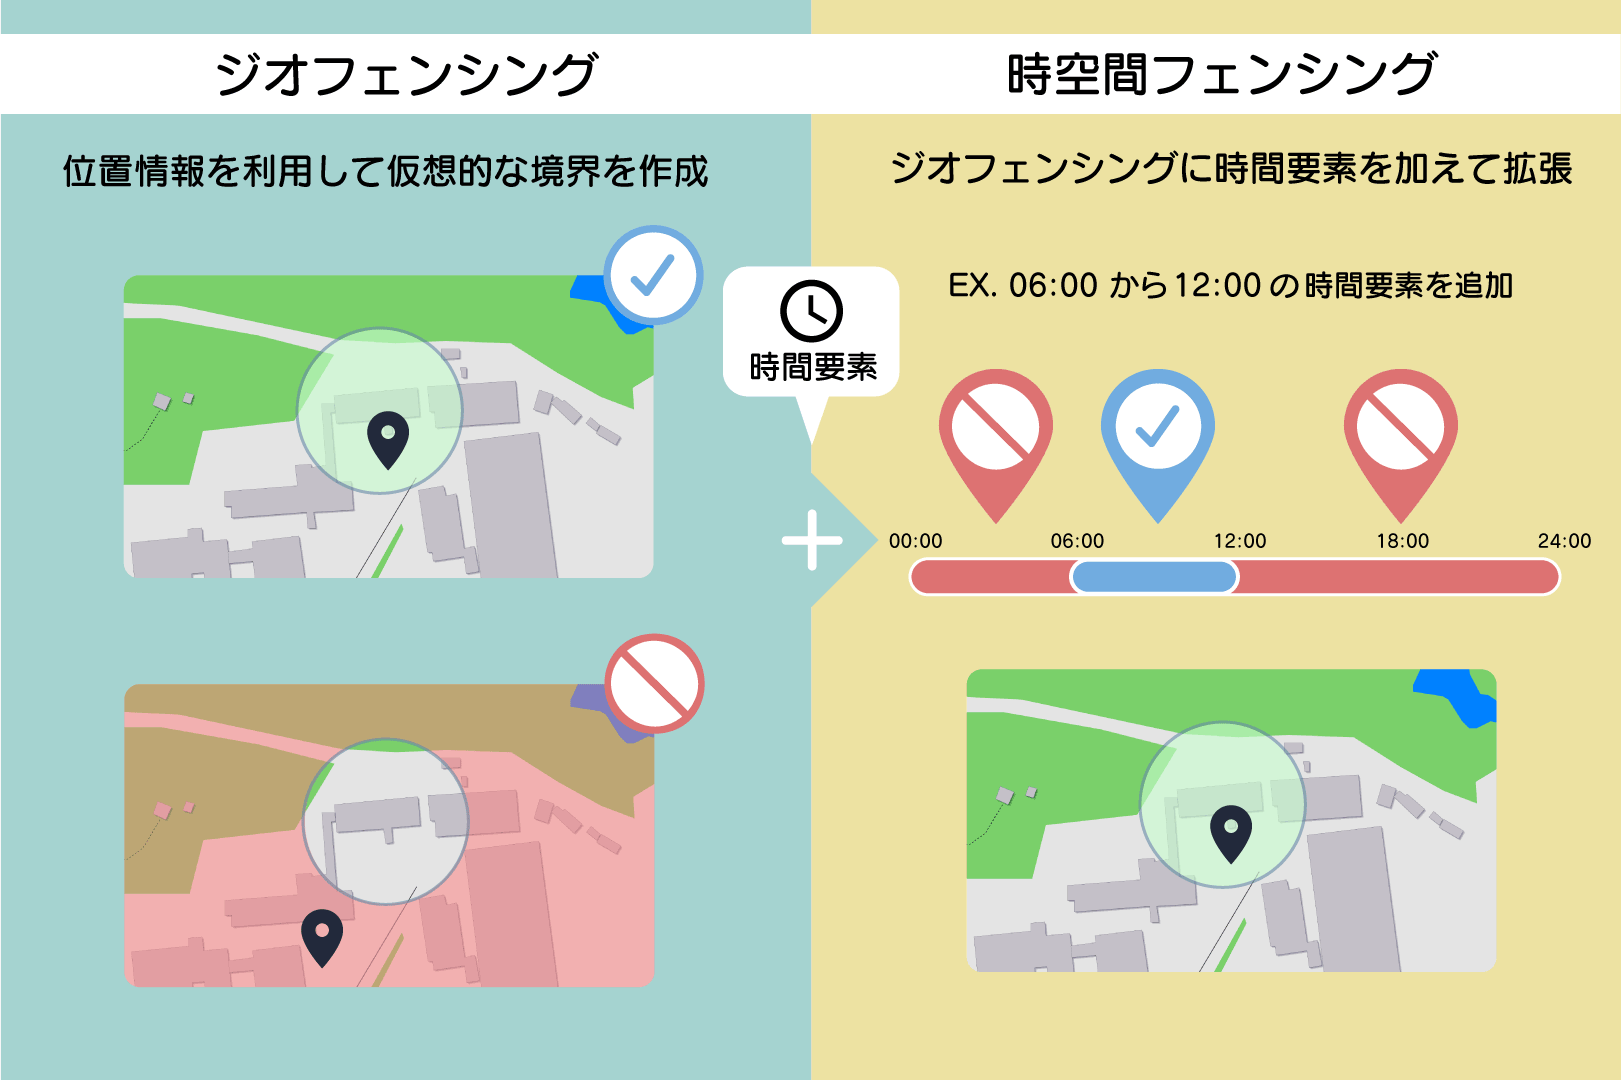
\includegraphics[width=150mm]{spatiotemporal.png}
    \caption{ジオフェンシングと時間要素を追加した時空間フェンシング}
    \label{fensing}
\end{figure}

時空間フェンシングは「ジオフェンシングに時間要素を追加し拡張したフェンシング手法」として定義する.
ジオフェンシングとはGPSやWi-Fi,BLEビーコンといった位置推定技術によって仮想的な境界を生成し,その境界に進入した,あるいは退出したときに特定のサービスを行うフェンシング手法である.
位置推定の高精度化や手軽にジオフェンスを構築できるBLEのようなデバイスの普及に伴って,ジオフェンシングを用いた様々なアプリケーションが実現されている.
つまり,時空間フェンシングとは,エリアと時間帯の指定によって仮想的な境界を生成し,その境界に進入した,あるいは退出したときに特定のサービスを行うフェンシング手法である.
特定のサービスとは,本研究では「センシング」である.
仮想的な境界内に進入したときにセンシングを開始し,境界外に退出したときにセンシングを終了する.

時空間フェンシングによって時間とエリアで境界を区切ると,依頼者は様々なシチュエーションを指定したクラウドセンシングが可能となる.
様々なシチュエーションとは,例えば「午後3時から5時の公園」であったり,「3限の1号館401教室」や「昼間の食堂」などである.
一方で,時空間フェンシングは時間やエリアに依存しないデータ収集には適さない.
例えば,一日中センシングを行なったり,電車で移動したりなどである.
このような長時間のセンシングやいつ終了するか定かではないセンシングは,協力者に消費電力など大きな負担をかけてしまう.
また,エリアのみ及び時間帯のみを指定するデータ収集には適さない.
エリアのみの場合,どこでセンシングされているかは分かっているが,いつセンシングされているかが明確ではない.
時間帯のみの場合も同様である.
依頼者と接点のない赤の他人が依頼者のセンシングに協力するとなった際,少しでもセンシング時間帯・エリアが曖昧であると,協力者は「協力しない」を選択する.
エリアと時間帯両方の明確な設定により,赤の他人のセンシングへの協力判断がしやすくする.
そのため本プラットフォームでは,依頼者が想定し得るすべてのセンシングに対応している訳ではない.
あくまでも時空間を指定したセンシングを想定している.

協力者のクラウドセンシングに対するプライバシ障壁は,時空間フェンシングによる時間とエリアの制限で軽減できる.
時間とエリアの指定がない場合,協力者は「いつどこでセンシングが開始し,終了するかわからない」という不安が生じるため,クラウドセンシングへの協力の判断がしにくい.
時間とエリアの指定がある場合,協力者は自分自身がプライベートな活動をしているのか,ある程度他人にデータ提供しても良い活動をしているのかを区別・判断しやすくなるため,クラウドセンシングへの協力の判断がしやすくなる.
時空間フェンシングにより,協力者は自分自身の可能な範囲内でセンシングに協力ができる.
% -----------------------------------------------
% -----------------------------------------------
% -----------------------------------------------

\section{ラヴラスの要求仕様}

本節では,ラヴラスにおける非機能要件を提示する.
3.2.1項では,ラヴラスにおけるクラウドセンシングプラットフォームとしての設計基盤について述べる.
3.2.2項では,協力者のプライバシ保護について述べ,3.2.3項では依頼者がラヴラスを利用する際の規約方針について述べる.
3.2.4項では,ラヴラスにおける利用者への配慮について述べる.
% -----------------------------------------------

\subsection{ラヴラスにおけるクラウドセンシングプラットフォームとしての設計基盤}
クラウドセンシングプラットフォームを構築するためには,一定の制限・制約を設計基盤として設ける必要がある.
この一定の制限・制約は,依頼者にとってクラウドセンシングの定義を簡略化でき,協力者にとっては受け入れやすいプラットフォームになるというメリットがある.
また,クラウドセンシングの実施方法に決まった手法や手順はなく,依頼者によって多種多様であるため,制限や制約はプラットフォームとして成立させるために必要不可欠な要素である.
関連研究として挙げた松田らの研究\cite{matsu}では,「ユーザ参加型モバイルセンシング基盤」という表現で我々のクラウドセンシングプラットフォームとしての設計基盤についての同様の記述がある.
松田らの研究では,ゲーミフィケーションによって協力者の協力へのモチベーションを向上させ,クラウドセンシングを行うための「シナリオ」がモジュール化されて定義されている.
それが我々のクラウドセンシングプラットフォームとしての設計基盤に相当する.
松田らの研究における「シナリオ」は,新規モジュールを開発し新たな「シナリオ」を追加はできるものの,モジュール化されていない「シナリオ」でのセンシングは出来ないという制約がある.

我々の構築するクラウドセンシングプラットフォーム「ラヴラス」のセンシングプラットフォームとしての設計基盤は,時空間フェンシングである.
我々が先ほど定義した時空間フェンシングを用いて,センシングを行う時間とエリアを制限するという制約を設けている.
時空間フェンシングをクラウドセンシングプラットフォームとしての設計基盤とすると,依頼者としては主に時空間フェンシングの設定とセンシングの設定の2つを定義すればいいため,容易にクラウドセンシングの定義が可能となる.
協力者としては,一定の時空間内でのみのセンシングであるため,プライバシの観点からクラウドセンシングへの協力を受け入れやすいといえる.

ラヴラスで実現しないセンシングは,時空間フェンシングでは適さないセンシングである.
例えば,一定の時間に依存しない1日の運動量といった長時間に渡るセンシングや時間に制限のない一定エリアでの活動のすべてといったセンシング,空間に依存しない車や電車等での移動中といったセンシングである.
これらは時空間内でのみセンシングという制限により,ラヴラスでは行わない.
また,時空間フェンシングの最大範囲を制限し,ラヴラスが定義する時間やエリアの範囲を超える時空間は定義できない.
これはエリアが市や県単位であったり,時間が「0時から24時」であった場合,制限がないのと同じになってしまうからである.
% -----------------------------------------------

\subsection{プライバシの保護}
世界的なインターネットの一般化によって,インターネットサービスを利用する際の個人データの取り扱いが重要となっている.
例えば,Facebookでは個人情報の不正流出が問題となり,2018年4月10日にCEOであるマーク・ザッカーバーグ氏が謝罪を行っている\cite{facebook}.
このような背景から,EUは個人データの取り扱いに対して,2018年5月25日にデータ保護指令(Data Protection Directive)に変わるGDPR(General Data Protection Regulation:一般データ保護規則)\cite{GDPR}を施行した.
GDPRは個人データやプライバシーの保護に関して,データ保護指令より厳格に規定し,制裁も強化している.

こういった国際的動向から,ラヴラスにおいてもプライバシの保護は必須である.
まず,設計基盤である時空間フェンシングという制限によって,時間やエリアの指定がないセンシングを実施しない.
また,時間やエリアを指定されている場合でも,依頼者の承諾なしでのセンシングは行わない.
これらにより,協力者の意図しないセンサのログデータ(以下,センシングデータ)の提供に伴うプライバシの侵害というリスクを最小限に抑える.
加えて,各協力者から提供されるセンシングデータやそれに結びつく端末情報などのセンシティブな情報を取り扱うため,依頼者のユーザ認証により,第三者による意図しないアクセスや情報の改ざんなどを防ぐ.

GDPRの個人データの定義(第4条)によると,協力者から提供される各センシングデータそのものは個人データには分類されないとされている.
しかし,そのセンシングデータに付随される情報との組み合わせによって,個人データに分類される可能性がある.
そのため,ラヴラスにはセンシングデータが個人情報となりえない設計が必要である.
例えば,協力者からのセンシングデータ提供の際,センシング行った環境情報として端末名やセンサの型番などの端末情報(以下,メタデータ)を取得するが,端末識別IDであるIMEI(International Mobile Equipment Identity)は個人データとなるため取得しない.
加えて,メタデータにはIMEI以外に,センシングデータとメタデータの参照により個人が識別可能になる場合,メタデータはセンシングを行った環境が判明する情報のみ取得するものとする.

さらに,協力者が特定のセンシングを拒否できる設計や提供したデータの削除要請を行う機能が必要がある.
上記で述べたように協力者から提供されるセンシングデータ及びメタデータは,個人情報に繋がらない特性情報のみに留めている.
しかし,協力者がプライバシを侵害されていると感じた場合,協力者の都合により特定のセンシングの拒否及び提供済みのセンシングデータ削除の要請などの要求に対応しなければならない.
依頼者側は協力者の協力拒否や削除要請の拒絶はできない.
これは,クラウドセンシングとは協力者ありきのデータ収集方法であり,協力者の信頼をなくしてしまっては成り立たないからである.
もし拒絶ができた場合,クラウドセンシングに対する信頼はなくなってしまい,協力者は該当のセンシングだけではなく,本プラットフォームの利用をやめてしまう可能性がある.
% 本プラットフォームは関連研究で述べたようなインセンティブを用いていないため,より協力者を第一に考えるプラットフォームでなければならない.
% -----------------------------------------------

\subsection{ラヴラスの利用規約方針}
依頼者はラヴラスを利用してクラウドセンシングを行う際,センシングの依頼(以下,センシングプロジェクト)を作成する必要がある.
センシングプロジェクトの作成を行うためには,依頼者の利用資格とそのセンシングプロジェクトを立ち上げる目的や使用センサ等のセンシングプロジェクトの内容の明示が必要である.
依頼者の利用資格を得るには,依頼者自身の情報が明示されている必要があり,匿名によるセンシングプロジェクトの作成はできない.
この依頼者情報は,基本的に依頼者本人の責任で保証されるものとし,ラヴラスでは登録されるメールアドレスが大学や所属機関のものかどうかなどの簡易的な確認のみを行うものとする.
センシングプロジェクトの内容の明示では,そのセンシングがどんな目的で行われるのか,センサはどんなものを使用するのか,実施期間や時空間フェンシングといった依頼内容を定義したものを明示する.
これは,どんな依頼者がどんな目的でデータ収集したいのかを明確にし,その実施内容が妥当なものであるのかを協力者が判断ができるようにするために必要である.
該当のセンシングプロジェクトの協力者にこれらの情報を明示し,協力者はその内容を了承した上でセンシングプロジェクトに協力する.

センシングデータの取り扱いの禁止事項として,「センシングデータの再利用禁止」と「保存期間以上のセンシングデータの保存禁止」を制定する.
センシングデータの再利用禁止は,「センシングデータの利用は依頼者本人(組織の場合はその組織)のみであるものとし,依頼者は収集したセンシングデータをそのプロジェクトに明示した目的を超える利用や第三者への開示・譲渡等は禁止する」と示す.
これは,協力者が依頼者のセンシングプロジェクトに同意した上で提供したセンシングデータが,協力者の意図と反して利用されてしまうからである.
ラヴラスが指定する保存期間以上のセンシングデータの保存の禁止は,「ラヴラスが定めるセンシングデータの保存期間を超える長期間の保存は禁止とする」と示す.
これは,センシングデータの提供方法をダウンロードとしているため,3.2.2項で述べた協力者による提供済みのセンシングデータの削除要請によって,削除されたセンシングデータが適切に利用できなくなるようにするためである.
センシングデータの提供方法をダウンロードとしているのは,依頼者が独自の環境で柔軟にセンシングデータの解析が行えるようにサポートするためである.
協力者による提供済みのセンシングデータの削除要請が行われたとき,直ちにサーバに保存された該当のセンシングデータの削除が行われるものとする.
しかし,削除要請以前に該当のセンシングデータが依頼者によってダウンロードされ,保存期間の終了前であった場合は,依頼者に該当のセンシングデータが削除要請によってサーバから削除されたと通知し,直ちに該当のセンシングデータの利用中止・削除を要請する.
このとき協力者の削除要請から依頼者が利用できなくなるまでにラグの発生が予想されるため,協力者に利用規約として提供済みのセンシングデータの削除要請が直ちに実行されるものではないと事前に通知する.
% -----------------------------------------------

\subsection{利用者への配慮}
ラヴラスの利用過程において負担となる要素がある場合,利用者は獲得しにくくなる.
そのため,利用者の視点から快適に利用できると思える配慮が必要である.
こうした配慮は,依頼者・協力者共に受け入れやすいプラットフォームを実現するために必要であり,依頼者と協力者が相互に利用しやすいプラットフォームを目指す上で重要となる.
本節では,心理的負担と物理的負担の2つの視点に分けて,その負担と配慮について述べる.

心理的負担としては,協力者がクラウドセンシングに協力する際に抱くプライバシを侵害されているという不安が挙げられる.
これは,協力者にとってスマートフォンから意図しないセンシングデータが提供されるかもしれないという不安ともいえる.
これに対する配慮として,安心してクラウドセンシングに協力できる環境を提案する必要がある.
まず,3.2.1項で挙げた時空間フェンシングによる時間とエリアによる制限がある.
協力者には,センシングプロジェクトに定義された時空間に進入した際にセンシングプロジェクトに協力するか否かを問う通知を送る.
協力者は,依頼内容や設定された時空間を確認した上で協力するかを判断し承諾された場合のみセンシングを行い,拒否した場合はセンシングは行わない.
このプロセスによって,協力者は意図したセンシングプロジェクトのみにセンシングデータの提供が可能である.
さらに,3.2.2項に挙げたように状況に応じてこのプロセスを通して承諾済みのセンシングプロジェクトの承諾取り消しや提供済みセンシングデータの削除が可能なため,誤って許可してしまったセンシングプロジェクトへの拒否や意図せず提供してしまったセンシングデータを削除もできる.

物理的な負担としては,1回のセンシング協力に伴う協力者の手間が挙げられる.
1回のセンシング協力にかかる手間が大きいほど,協力者のセンシング協力に対するモチベーションは低下し,継続的なセンシング協力は得られにくい.
これに対する配慮として,協力者の手間となるスマホアプリの操作は,基本的に上記に記した通知画面よりセンシングプロジェクトへの承諾及び拒否を行うのみで行えるように設計する.
この操作は協力するセンシングプロジェクトごとに初めの1回のみであるため,再度同じセンシングプロジェクトに設定された時空間に進入した場合は一切操作は行う必要はなく,自動的にセンシングを開始する.
また,センシングの終了や終了後のセンシングデータのアップロードは自動で行われるため,協力者がスマホアプリを操作する必要はない.
さらに,センシングデータのアップロードはWi-Fi環境下のみで行うため,協力者のパケット通信量を最小限に抑える.
この他に,依頼者・協力者に共通してラヴラスを利用する際に必要不可欠なユーザインターフェイスについても配慮を行う.
ユーザインターフェイスは,利用者によって使いやすさに直結するものである.
情報の表示や入力のしやすさが低ければ,利用者によって物理的負担となり利用されにくいプラットフォームとなるためである.
% -----------------------------------------------
% -----------------------------------------------
% -----------------------------------------------
% -----------------------------------------------

\section{ラヴラスの実装}
先述のプラットフォームの要求仕様に則って,クラウドセンシングプラットフォーム「ラヴラス」の実装を行う.
本プラットフォームは,センシングデータの管理や各プロジェクトを管理するサーバ,依頼者専用のプロジェクトの作成・管理を行うWebアプリ,協力者専用のセンシングを行うスマホアプリによって構成する.
3.3.1項では,依頼者と協力者がラヴラスを操作する際の手順について述べる.
3.3.2項では,センシングデータの管理や各プロジェクトを管理するサーバの実装について述べる.
3.3.3項では,依頼者専用のセンシングプロジェクト管理やセンシングデータダウンロードを行うWebアプリの実装について述べる.
3.3.4項では,協力者専用のセンシングスマホアプリの実装について述べる.
% -----------------------------------------------


\subsection{ラヴラスの操作手順}

\begin{figure}[H]
    \centering
    \includegraphics[width=150mm]{fig1.png}
    \caption{ラヴラスによるクラウドセンシングの操作手順}
    \label{fig:1}
\end{figure}

ラヴラスの一連の流れは「Webアプリでセンシングプロジェクトの定義」,「時空間フェンシング」,「センシング依頼の承諾」,「自動的にセンシング」,「Wi-Fi環境下で自動的にアップロード」,「データ利用」の順で行う(図\ref{fig:1}).
依頼者側では「Webアプリでセンシングプロジェクトの定義」と「データ利用」が行われる.
一方で,協力者側では「時空間フェンシング」,「センシング依頼の承諾」,「自動的にセンシング」,「Wi-Fi環境下で自動的にアップロード」が行われる.
ラヴラスを利用してクラウドセンシングを行う際のユーザの使用デバイスとして,依頼者はPCを,協力者はスマートフォンを前提としている.
依頼者がラヴラスを利用するためには,まずWebアプリでユーザ登録してもらう.
協力者がラヴラスのクラウドセンシングに協力するためには,ラヴラス専用のスマホアプリをインストールしてもらう.

依頼者はプロジェクト管理Webアプリにて,センシング依頼の内容を細かく定義し,センシングプロジェクトを作成する.
センシングプロジェクトとはセンシングを行いたい時間帯やエリア,センシングを行う目的,概要,センシングに用いるセンサの種類やそのセンサのサンプリングレートなどである.
これは協力者側のスマホアプリでセンシングや時空間フェンシングの設定に必要であるとともに,協力者にセンシングプロジェクトを提示し,協力するか否かの判断材料にしてもらう.
作成されたセンシングプロジェクトはスマホアプリ側が適宜取得し,取得したプロジェクトに応じて時空間フェンシング・センシング依頼通知・センシングを行う.

スマホアプリ側ではセンシングプロジェクトに応じて,3.1節の定義をもとに時空間フェンシングを行い,協力者が指定された時間帯かつエリアにいる場合のみ通知が送られる.
そのため,時間帯・エリアのどちらか一方のみ当てはまる場合は通知は送られない.
例えば,指定エリア内に進入していたとしても,指定時間帯に入っていない及び過ぎている場合は通知は送られない.
指定時間帯に入っていて,指定エリア内に進入していない場合も同様である.
また,時空間フェンシングはバックグラウンドで行うため,本スマホアプリを開いておく必要はない.
そして,指定された開始時間から終了時間の間であれば,いつ指定されたエリアに進入しても通知は送られる.
指定されたエリアを退出し,一定時間後再び進入した場合は,通知を送らずにセンシングを開始する.

\begin{figure}[H]
  \centering
  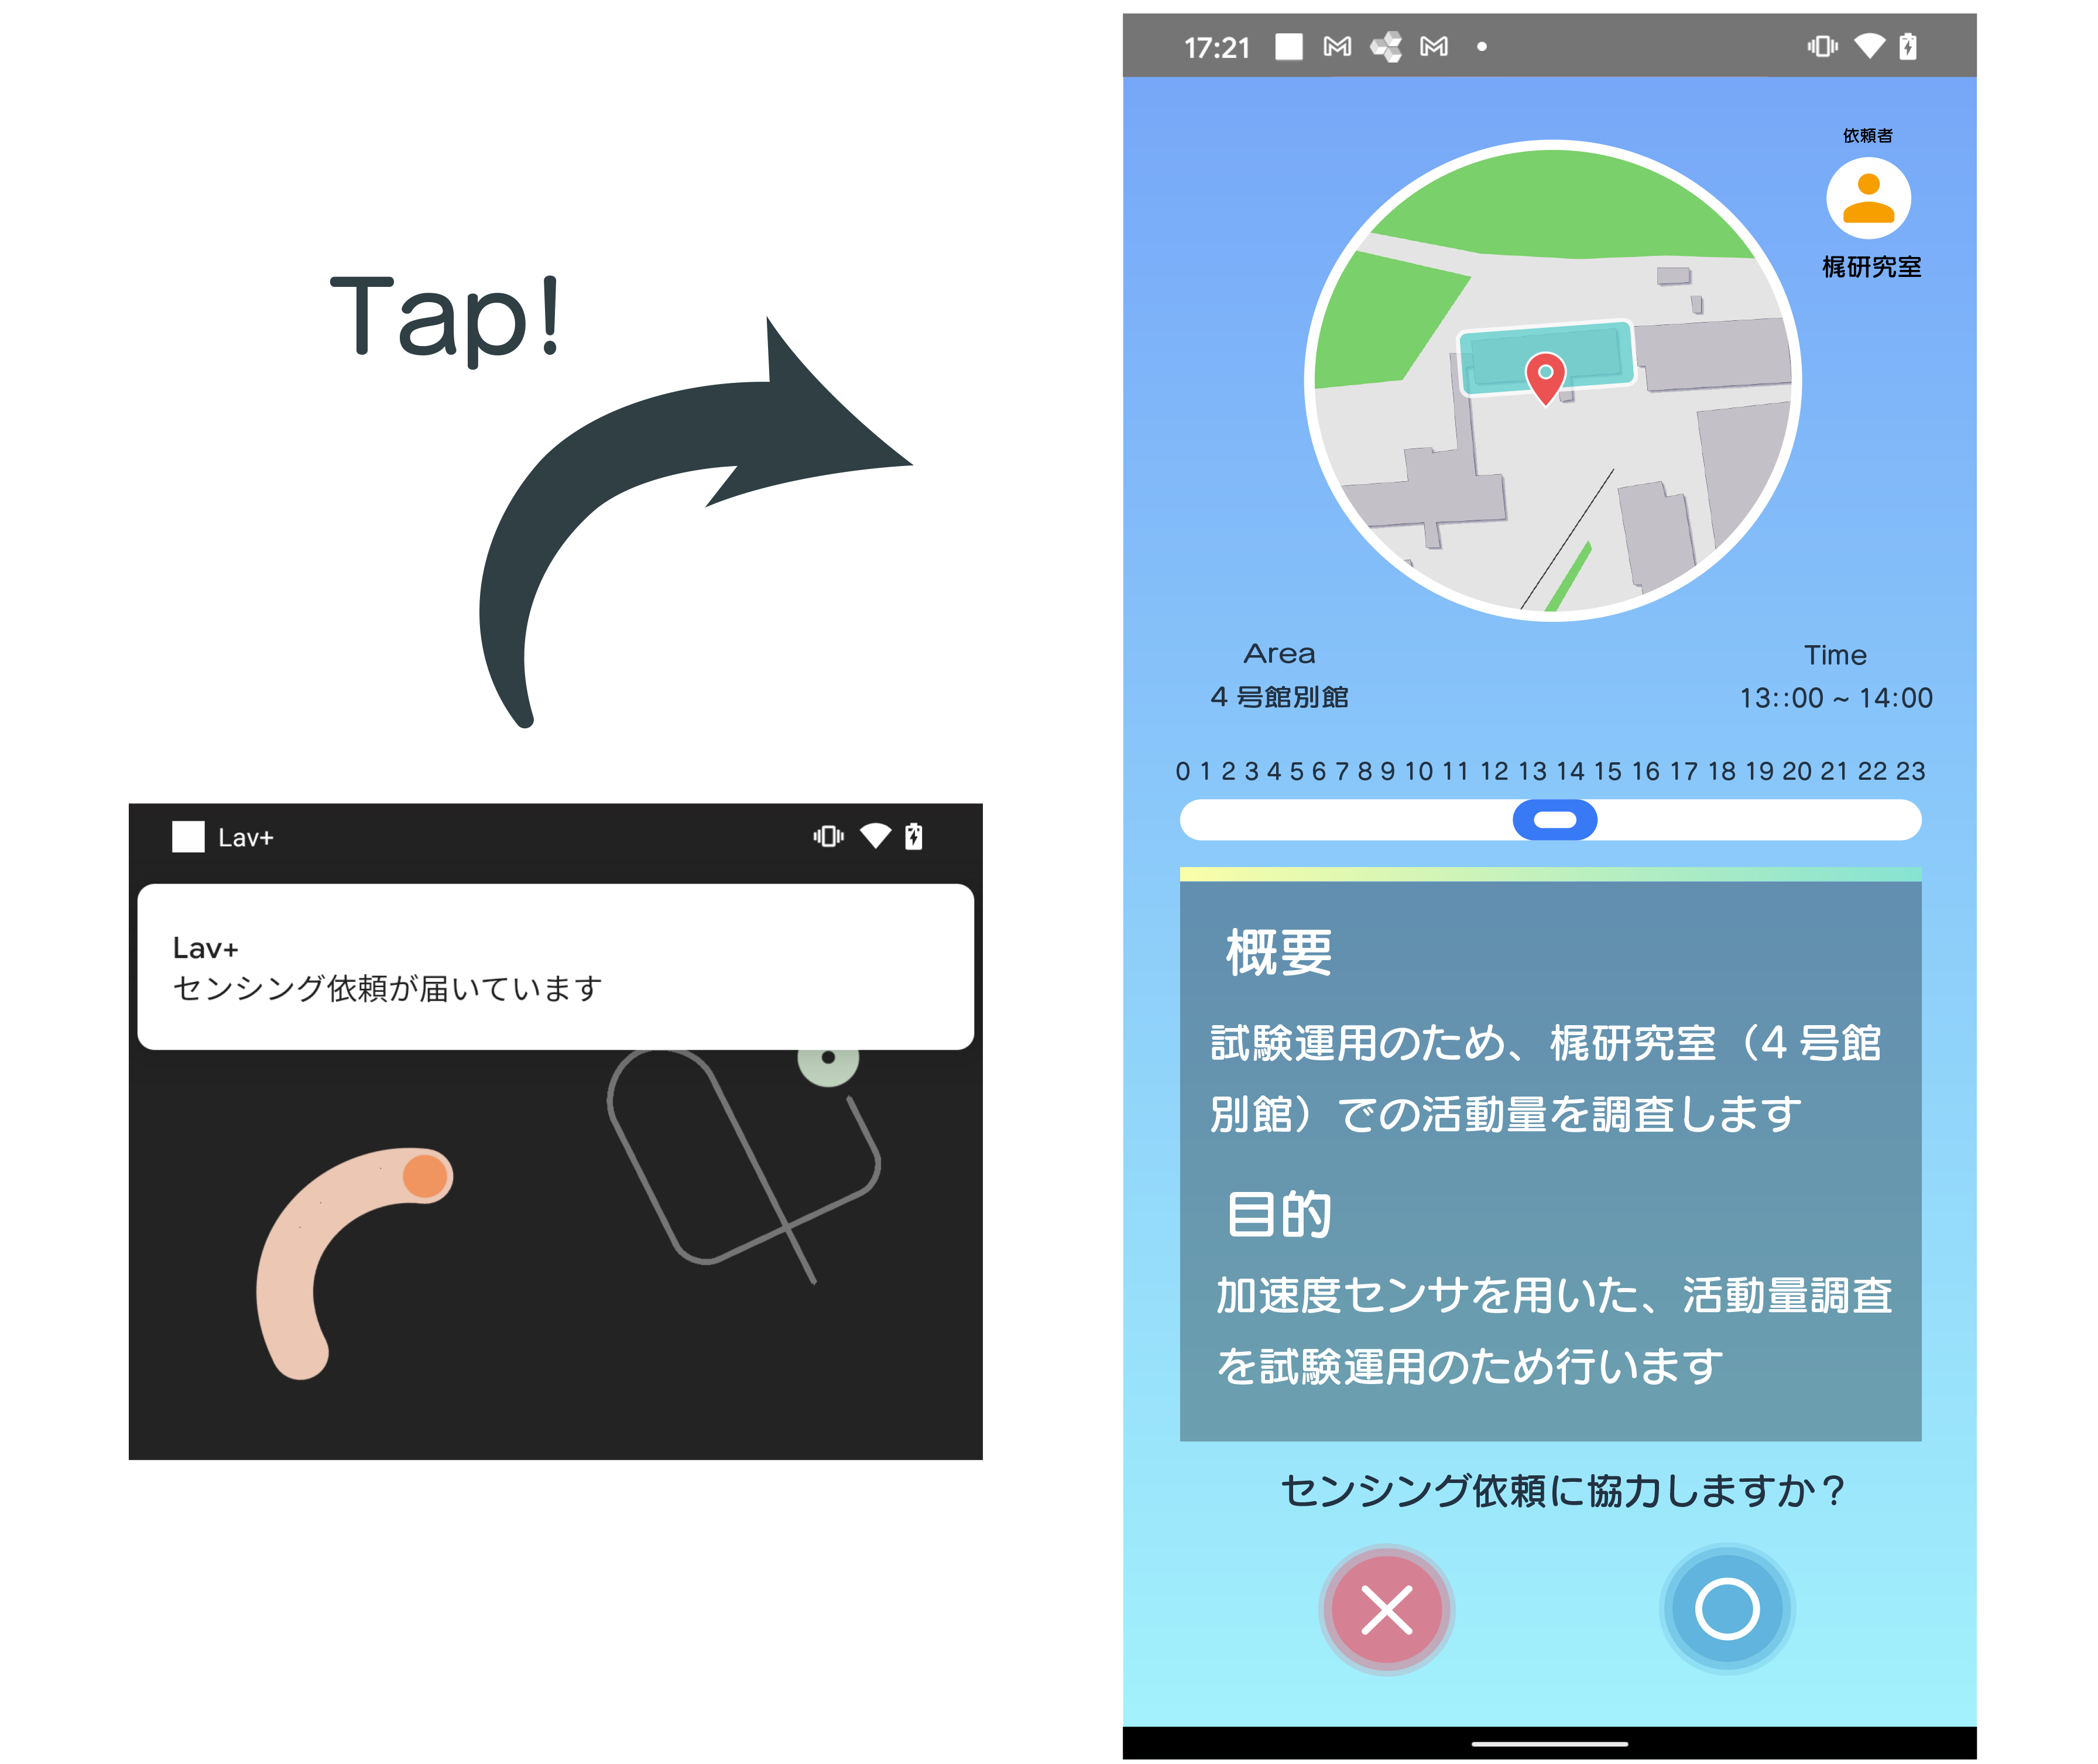
\includegraphics[width=100mm]{fig2.png}
  \caption{センシング依頼のヘッドアップ通知と通知画面}
  \label{fig:2}
\end{figure}

協力者はヘッドアップ通知のクリックで本アプリケーションの通知画面を開き,依頼されているセンシングプロジェクトの内容を確認し,承諾・拒否の判断をする.
通知画面で表示する情報としては,センシングを行うエリア,時間帯,センシングの目的,概要,依頼者の情報である.
また,時空間内に進入した際の現在地と指定エリアをGoogle Mapsで位置関係をより分かりやすく表示している.
センシング依頼の内容に納得し,協力してもいい場合に承諾ボタン(通知画面では丸ボタン)を押す.
そうすると,センシングが開始される.
通知が届いた時間帯やエリアが協力者にとってセンシングされたくない時間またはエリアの場合,または届いたセンシング依頼に協力したくない場合は,拒否ボタン(通知画面ではバツボタン) を押す.
そうすると,センシングは開始せずに終了する.
ラヴラスのクラウドセンシングの手順において協力者がスマートフォンを操作するのは主にこの通知から承諾・拒否の部分である.
承諾ボタンを押したら,もうスマホアプリは閉じても構わない.

センシングも常にバックグラウンドで行うため,アプリケーションを開いておく必要はない.
バックグラウンドでのセンシングにより,協力者がセンシング終了するなどの操作をする必要がない.
センシング終了後はWi-Fi接続時にのみ自動でサーバ側にアップロードされる.
協力者のスマートフォンがWi-Fiなどに接続されている場合にセンシングデータをサーバにアップロードする.
接続されていない場合は,アップロードせずディレクトリに格納しておき,Wi-Fiなどに接続された際にまとめてアップロードする.

依頼者は本Webアプリにて,アップロードされたセンシングデータを閲覧可能である.
% -----------------------------------------------

\subsection{センシングデータの管理や各プロジェクトを管理するサーバの実装}

センシングデータの管理や各プロジェクトを管理するサーバは,Webアプリ及びスマホアプリのどちらからの連携もスムーズ行えるようにそのどちらにも親和性が高いJSONベースのREST APIとして設計した.
REST APIとしてサーバを設計すると,MVCモデルにおけるModelとControllerをView部分にあたるWebアプリとスマホアプリを完全に分離し,実装の分業化及びオブジェクト指向設計の原則における単一責任の原則によって,各機能のカプセル化を実現し,メンテナンスや拡張実装をより柔軟にするという狙いもある.
サーバは,構築する上でJSON形式のファイルを取り扱いやすい言語を選択する必要があったため,JavaScript(Node.js)を選択した.
また,JavaScriptはJSONファイルをよりネイティブに取り扱いやすい言語であり,REST API専用のフレームワークの選択肢が他言語に比べて多く存在している.
REST APIのフレームワークは,Webサーバ系フレームワークとして有名なExpressを,REST API専用のフレームワークとして再設計されたLoopBack4を採用した.
サーバで使用するデータベースは,今後のスマートフォンのさらなる高性能化による搭載センサの種類増加に伴うデータベースの変更やシステムの拡張性の向上を図るため,変更や操作が柔軟に可能なデータベースとしてNoSQLデータベースのMongoDBを採用した.

サーバのデータベースとREST APIのエンドポイントを3.2節「ラヴラスの要求仕様」を基に設計を行った.
NoSQLデータベースであるMongoDBにはリレーショナルデータベースにおけるテーブルのカラムの概念が存在しないため,各モデルの定義をLoopBack4のモデルによって定義する.
以下の各モデルの説明には,LoopBack4で定義したモデルによって作成したコレクション(リレーショナルデータベースにおけるテーブルに相当)とそのコレクション内のドキュメント(リレーショナルデータベースにおけるレコードに相当)の一例を示すものとする.

\begin{figure}[H]
  \centering
  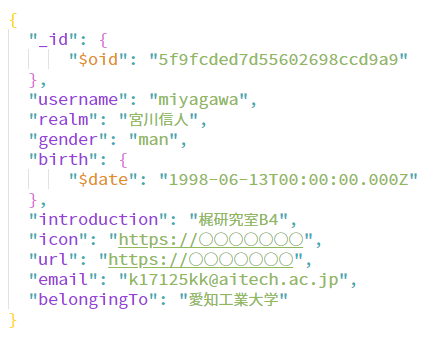
\includegraphics[width=96mm]{User.png}
  \caption{Userコレクションのドキュメント一例}
  \label{User}
\end{figure}

各依頼者を管理するためのモデルとしてUserモデル(図\ref{User})を定義した.
Userモデルには,ドキュメント管理用の「id」,ユーザ名「username」,依頼者の本名「realm」,性別「gender」,生年月日「birth」,紹介文「introduction」,アイコン画像「icon」,eメールアドレス「email」,Webページリンク「url」,所属機関「belongingTo」の10項目を定義した.
要求仕様の3.2.3項「ラヴラスの利用及び利用規約の方針」に基づき,依頼者の利用資格の観点から匿名によるセンシングプロジェクトの作成はできないため,ユーザ名,依頼者の本名,性別,生年月日,eメールアドレス,所属機関を必須項目として設定を行った.
REST APIのエンドポイントは,ユーザ登録を行う「/singup(POST)」,ログイン用の「/users/login(POST)」,ログイン後自身の情報を取得する「/whoAmI(GET)」を作成した.

\begin{figure}[H]
  \centering
  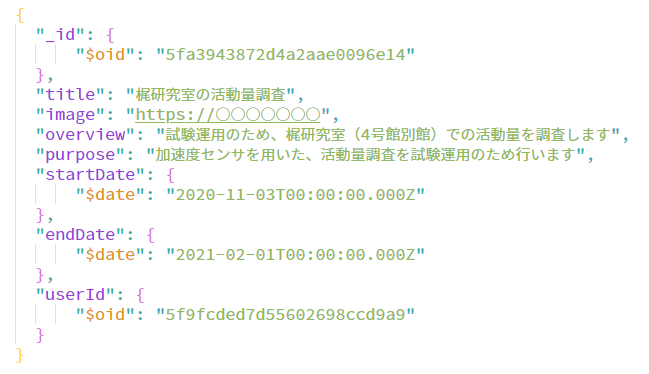
\includegraphics[width=120mm]{Project.png}
  \caption{Projectコレクションのドキュメント一例}
  \label{Project}
\end{figure}

各センシングプロジェクトを管理するためのモデルとしてProjectモデル(図\ref{Project})を定義した.
Projectモデルには,ドキュメント管理用の「id」,プロジェクトタイトル「title」,サムネイル用画像「image」,概要説明「overview」,目的「purpose」,センシングプロジェクトの開始日「startDate」と終了日「endDate」,作成したUserのid「userId」の8項目を定義した.
REST APIのエンドポイントは,「/project」でそれぞれの操作に対応するHTTPメソッドによりCRUD操作(Create,Read,Update,Delete)が可能となる.
これらの項目のうちサムネイル用画像以外の項目はすべて必須項目であり,要求仕様の3.2.3項「ラヴラスの利用及び利用規約の方針」に基づき,センシングプロジェクトの内容を明確にするために概要や目的の説明文の項目を定義している.
また,同要求仕様に示されたセンシングに関するセンサの定義や時空間フェンシングの定義は,SensingSettingモデルで定義を行っている.
センシングプロジェクト作成に必要な情報をProjectモデルとSensingSettingモデルに分離するのは,スマホアプリがSensingSettingモデルのエンドポイントから各センシングプロジェクトのセンシングに関する設定を直接的な読み込みを可能にするためである.

\begin{figure}[H]
  \centering
  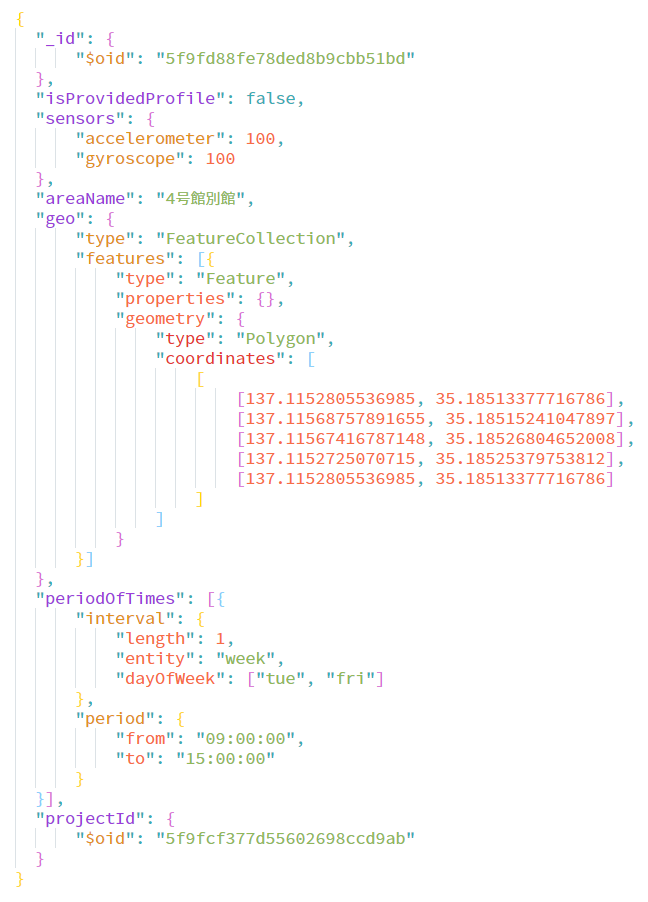
\includegraphics[width=120mm]{SensingSetting.png}
  \caption{SensingSettingコレクションのドキュメント一例}
  \label{SensingSetting}
\end{figure}

SensingSettingモデル(図\ref{SensingSetting})には,ドキュメント管理用の「id」,協力者に自身の基礎情報(身長・体重・性別など)を求めるか否かの設定「isProvidedProfile」,使用センサの種類とそれぞれのセンサのサンプリングレート(Hz)「sensors」,時空間フェンシングのエリア名「areaName」,GeoJSONによる時空間フェンシングのエリア設定「geo」,時空間フェンシングの時間帯設定「periodOfTimes」,紐づくセンシングプロジェクトのid「projectId」の7項目を定義した.
REST APIのエンドポイントは,「/sensing-setting」でそれぞれの操作に対応するHTTPメソッドによりCRUD操作が可能となる.
協力者に自身の基礎情報を求めるか否かの設定「isProvidedProfile」は,依頼者がセンシング協力を行う協力者の体格や性別に応じた変化を含めて調査を行いたい場合に利用するための項目として定義した.
これは,協力者に基礎情報の登録をスマホアプリで行ってもらい,その情報をセンシングデータと共に送信するものであるが,現在実装には至っていないため定義のみとする.
時空間フェンシングの定義として,柔軟に依頼者の想定するシチュエーションに対応するためには,複数のエリアや異なる時間帯を定義できるフォーマットにする必要がある.
時空間フェンシングのエリア設定「geo」は,現在のエリア判定方法がGPS情報による判定でのみであるため,地理的データを表現するフォーマットであるGeoJSON形式を用いてエリアの設定を行っている.
エリアの定義にGeoJSON形式を用いた理由は,2つ以上のエリアの定義を可能にできる他,複雑なエリアの指定も可能にするためである.

\begin{figure}[H]
  \centering
  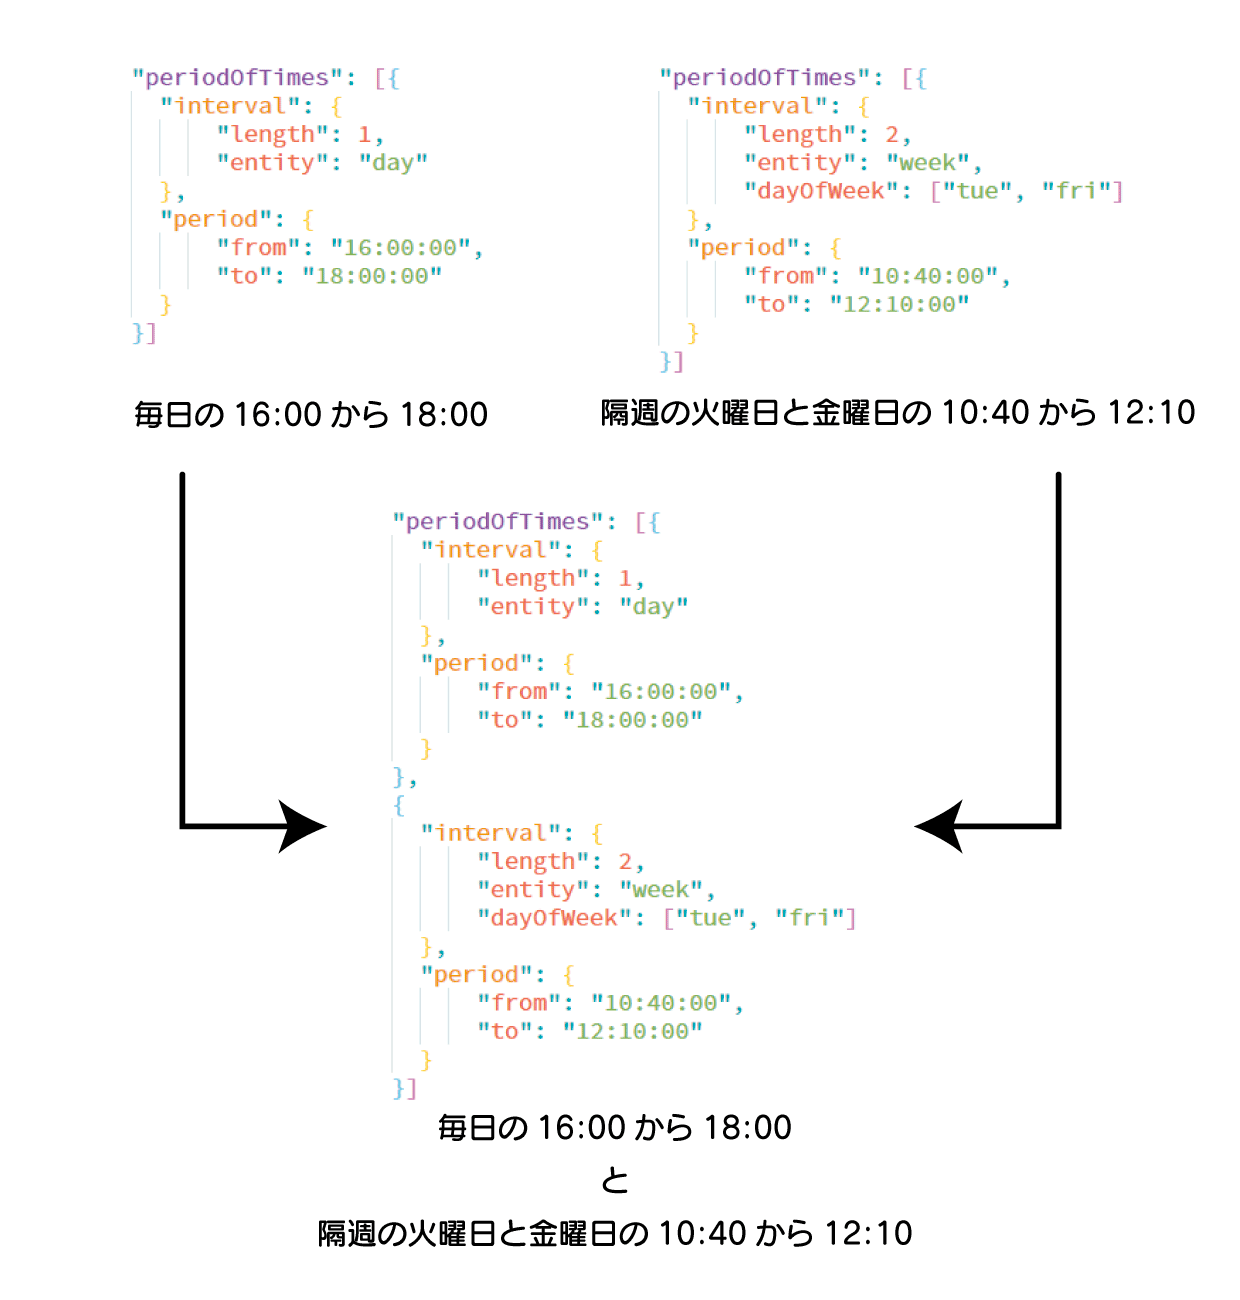
\includegraphics[width=150mm]{periodOfTimes.png}
  \caption{periodOfTimesの定義の例}
  \label{periodOfTimes}
\end{figure}

時空間フェンシングの時間設定「periodOfTimes」も,複数の時間帯を定義可能なフォーマットを定義した(図\ref{periodOfTimes}).
このフォーマットは,intervalとperiodからなるオブジェクトの配列として定義する.
intervalは,指定された時間帯を繰り返す間隔を定義するプロパティでlength,entity,dayOfWeekからなるオブジェクトである.
entityとdayOfWeekは間隔を設ける単位を表現し,entityには"day"もしくは"week"のどちらかのテキストが入り,"day"の場合はdayOfWeekプロパティが省略され,"week"の場合はdayOfWeekプロパティに指定する曜日を3文字の曜日の省略表記を用いて文字列の配列として定義する.
lengthには,数字を指定しentityとdayOfWeekで指定した単位で間隔を設ける.
periodは,fromプロパティにセンシング開始時間,toプロパティにセンシング終了時間を指定する.
このフォーマットによって例えば,「毎日の16:00から18:00まで」や「隔週の火曜日と金曜日の10:40から12:10」といった指定やその両方の指定が可能になる.

\begin{figure}[H]
  \centering
  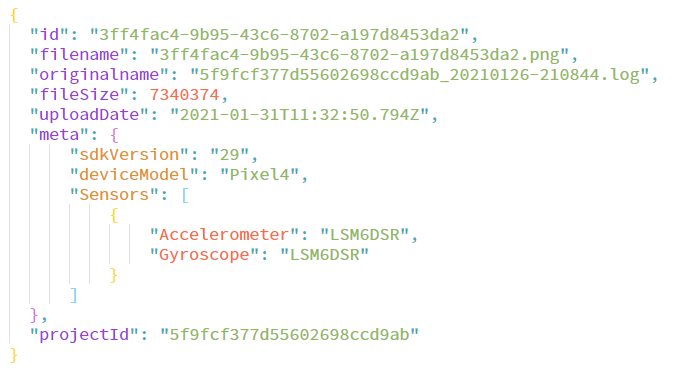
\includegraphics[width=120mm]{SensingData.png}
  \caption{SensingDataコレクションのドキュメント一例}
  \label{SensingData}
\end{figure}

協力者によって提供される各センシングデータを管理するモデルとしてSensingDataモデル(図\ref{SensingData})を定義した.
SensingDataモデルには,ドキュメント管理用の「id」,サーバ内部で保存したファイル名「filename」,協力者から提供されたオリジナルのファイル名「originalname」,ファイルのサイズ(byte)「fileSize」,アップロードが行われた日時「uploadDate」,メタデータ「meta」,提供されたセンシングプロジェクトのid「projectId」の7項目を定義した.
REST APIのエンドポイントは,「/sensing-data」でそれぞれの操作に対応するHTTPメソッドによりCRUD操作が可能となる.
オリジナルのファイル名を変更しサーバで保存を行っているのは,サーバ内で同名のファイルが保存され上書きされる可能性があるためである.
また,メタデータは要求仕様の3.2.2項「プライバシの保護」に基づき,個人データに該当しないOSのSDKバージョン,デバイスモデル,使用したセンサとその型番のみを取得する.
センシングデータをアップロードするための専用のエンドポイントとして,「/sensing-data/upload(POST)」を作成する.
このエンドポイントは,バイナリデータであるセンシングデータを取り扱うためにJSON形式によるエンドポイントではなく,「multipart/form-data」を使用し,スマホアプリがセンシングデータのアップロードと「/sensing-data」を通してセンシングデータの情報のアップロードを行う手間を削減するために,センシングデータがアップロードされるとサーバは自動的にSensingDataコレクションにドキュメントを作成する.

\begin{figure}[H]
  \centering
  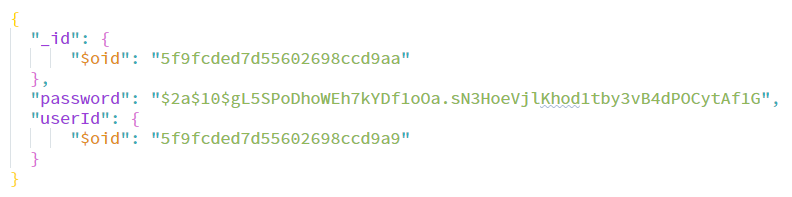
\includegraphics[width=150mm]{UserCredentials.png}
  \caption{UserCredentialsコレクションのドキュメント一例}
  \label{UserCredentials}
\end{figure}


最後に,要求仕様の3.2.2項「プライバシの保護」に対応するためのセキュリティ対策としてJWTトークン認証を導入した.
JWTトークン認証を実現するために,Userモデルに結びつき認証情報を保持するUserCredentialsモデル(図\ref{UserCredentials})を定義した.
UserCredentialsモデルには,ドキュメント管理用の「id」,依頼者が設定したパスワードのハッシュ値「password」,結びつくUserモデルのid「userId」の3項目で定義される.
セキュリティ対策として依頼者の設定したパスワードは,そのままの値で保持せずハッシュ値を用いている.
このJWTトークン認証によって各エンドポイントの不正なアクセスの防止を実現する.
例えば,提供済みのセンシングデータのダウンロードを行うエンドポイントは,センシングプロジェクトの作成を行った依頼者本人でなければアクセスができない.
図\ref{fig401}は,権限の無いユーザがセンシングデータのダウンロードを行うためのエンドポイントにアクセスした際に表示されるエラーメッセージである.



\begin{figure}[H]
  \centering
  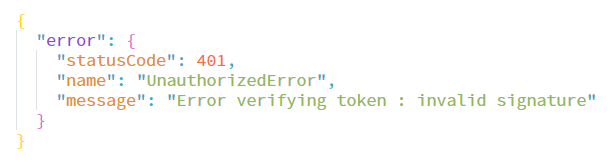
\includegraphics[width=120mm]{401.png}
  \caption{権限の無いユーザがセンシングデータのダウンロードを試みる例}
  \label{fig401}
\end{figure}

% -----------------------------------------------

\subsection{依頼者用のプロジェクト管理Webアプリの実装}

\begin{figure}[H]
  \centering
  \includegraphics[width= 150mm]{serverAndWeb.png}
  \caption{サーバとWebアプリの連携}
  \label{kanri}
\end{figure}

依頼者のユーザ登録やセンシングプロジェクトの作成及び管理を行うためのWebアプリには,Single Page Application(以下,SPA)を採用し実装を行った.
SPAは,その名前にシングルページとあるように単一のHTMLをJavaScriptを用いた動的な変更により,画面を描画するWebアプリのアーキテクチャである.
SPAを用いるとJavaScriptによってページを制御できるため,デスクトップアプリケーションのような操作を実現できる他,REST APIとの親和性も高くサーバとの連携に柔軟に対応できる.
依頼者用のインターフェイスとして,Webアプリを採用する.
これにより環境依存が少なく,SPAによってデスクトップアプリケーションに近い操作感を得られるため,要求仕様の3.2.4項「利用者への配慮」のユーザインターフェイスへの配慮を実現している.
また,SPAのフレームワークにはコンポーネントベースでSPAを作成できるReactを採用した.
コンポーネントベースとは,ヘッダやボタンといったパーツをコンポーネントという単位で作成し,それらを組み合わせによってSPAを作成する設計思想である.
コンポーネントベースのReactの採用により,作成したコンポーネントの再利用や修正・管理がしやすくなる.
また,コンポーネント単位ですべてのパーツを管理できるため,拡張性やメンテナンス性の向上,開発工数の削減が期待できる.
 
\begin{figure}[H]
  \centering
  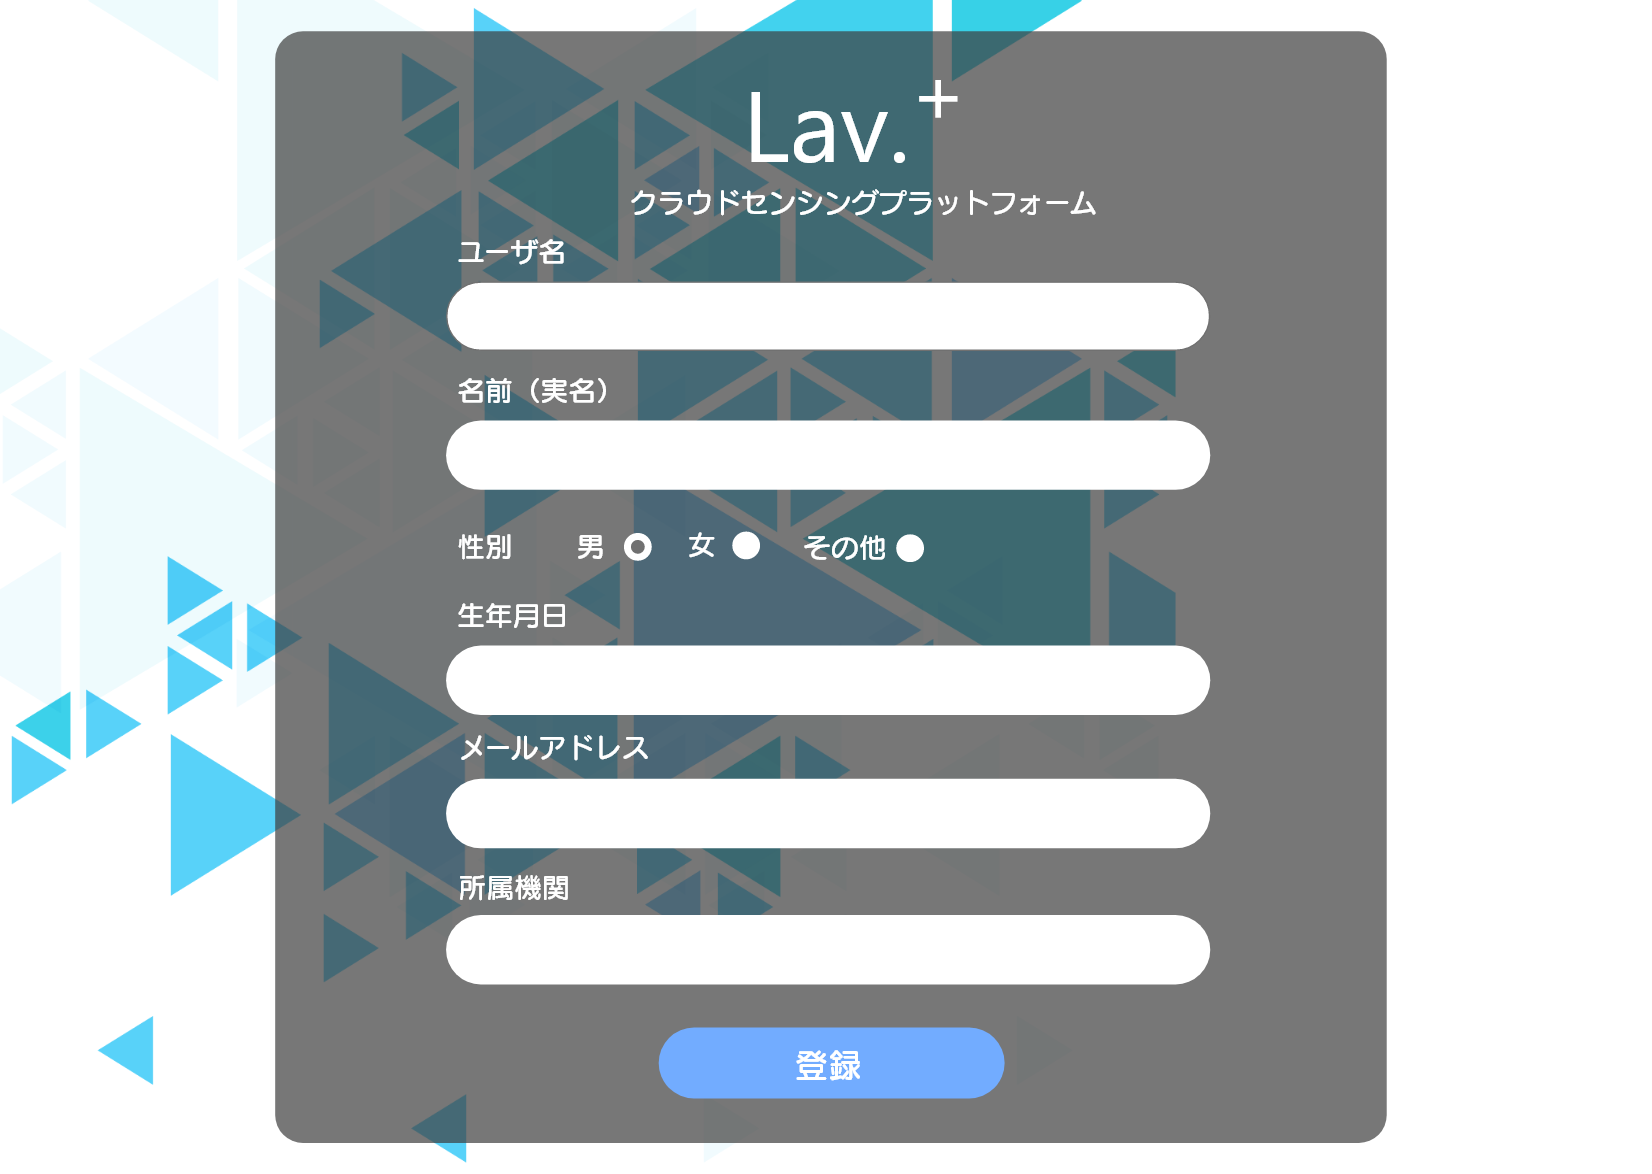
\includegraphics[width=120mm]{Signup.png}
  \caption{ユーザ登録画面}
  \label{baseSetting}
\end{figure}

Webアプリでは,まず依頼者がユーザ登録を行う.
ユーザ登録では,サーバのUserモデルに合わせたフォームを作成し要求仕様の3.2.3項「ラヴラスの利用及び利用規約の方針」に基づき本名,性別,生年月日,eメールアドレス,所属機関の5項目を必須項目とする.
入力が完了し送信ボタンのタップにより,サーバの「/singup」エンドポイントに入力情報が送信され登録完了となる.
次に,新規センシングプロジェクトを作成する.
センシングプロジェクトの入力フォームは入力項目が多いため,要求仕様の3.2.4項「利用者への配慮」のユーザインターフェイスの配慮に対応し,「基本設定」「概要と目的」「有効期限」「センサ設定」「時空間フェンシング設定」の項目の5ページに分け,さらに入力の複雑な項目に対して入力操作を簡易化する仕組みで入力操作の向上を図っている.
各ページの右上に前のページに戻るボタン,入力フォームの下部に次の入力項目に遷移するためのボタンを設置する.
これらのページは,遷移を行っても内部的に入力されたフォームの情報を保持しており,入力を前のページに戻り修正が可能である.
% (img baseStting.png cap: 基本設定ページの入力画面と入力例)
\begin{figure}[H]
  \centering
  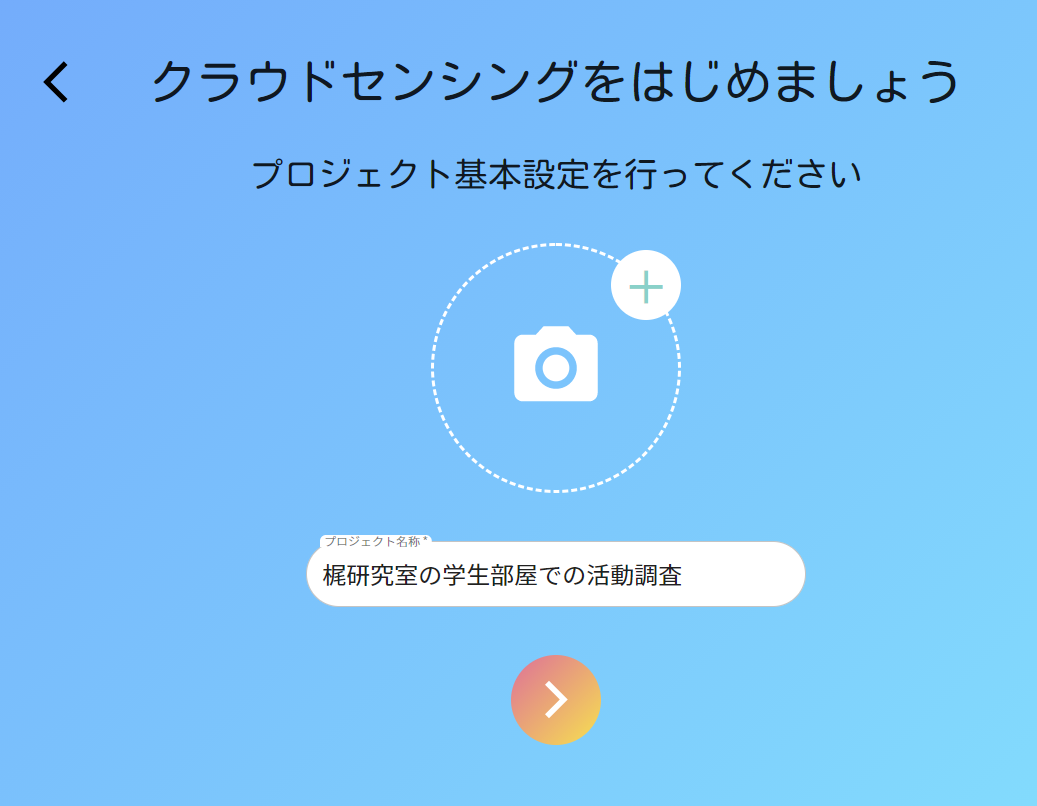
\includegraphics[width=80mm]{baseSetting.png}
  \caption{基本設定ページの入力画面と入力例}
  \label{baseSetting}
\end{figure}

基本設定ページ(図\ref{baseSetting})では,サムネイル用画像とセンシングプロジェクトの名称の入力を行う.
この入力ページでは,プロジェクトの名称のみが必須項目であるため,サムネイル用画像は任意とする.
この2つの項目は,サーバに定義されたProjectモデルの「title」と「image」に対応している.
% (img overview.png cap: 概要と目的ページの入力画面と入力例)
\begin{figure}[H]
  \centering
  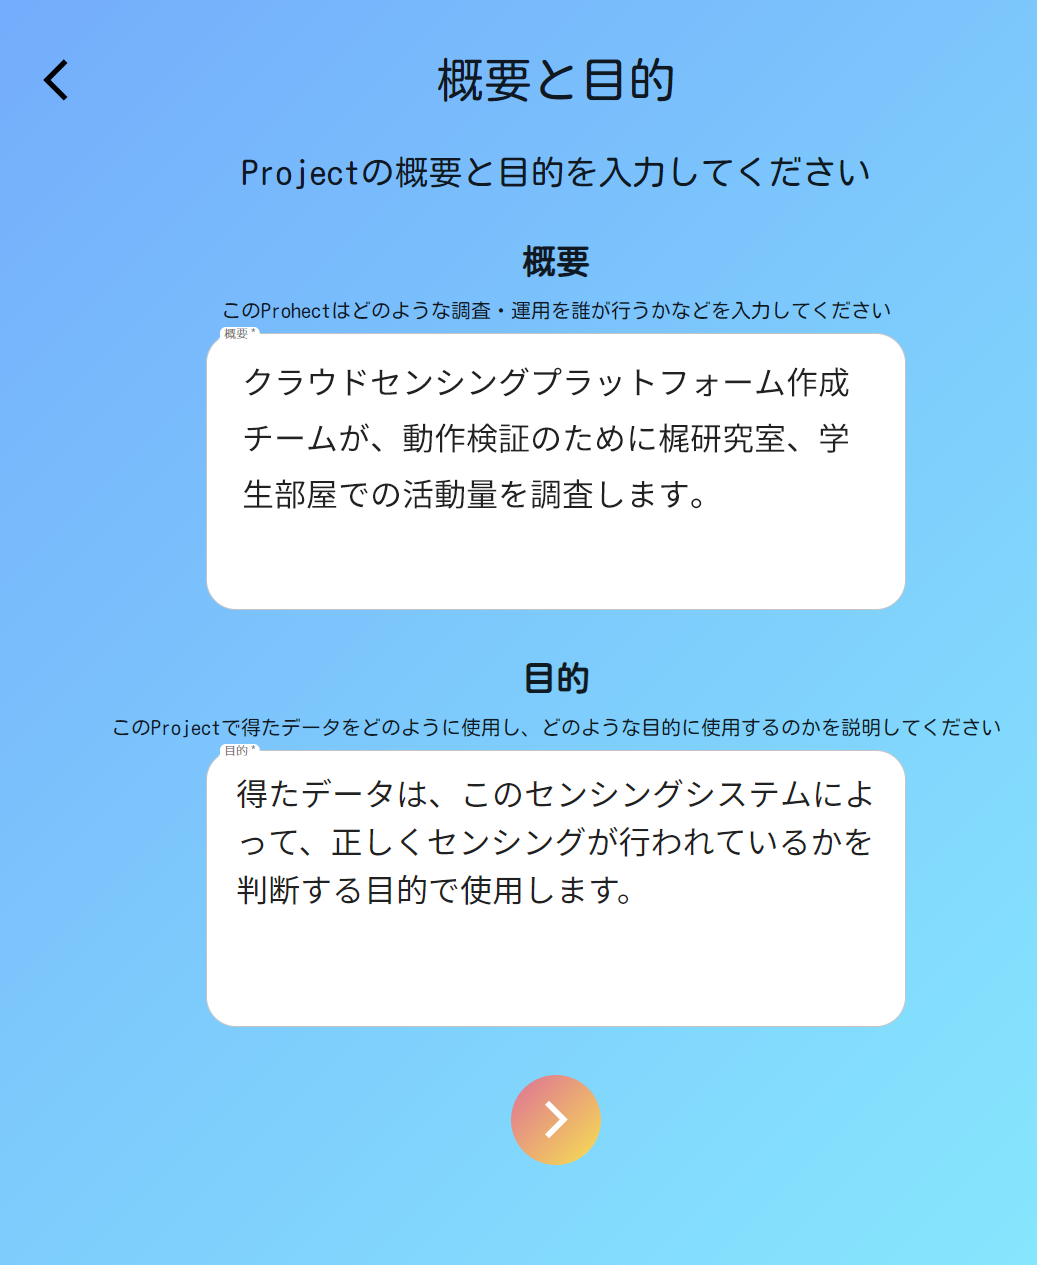
\includegraphics[width=80mm]{overview.png}
  \caption{概要と目的ページの入力画面と入力例}
  \label{overview}
\end{figure}

概要と目的ページ(図\ref{overview})では,概要と目的の入力を行う.
この入力ページでは,どちらの入力項目も必須項目であり,最低文字数20文字以上の入力が必要となっている.
この2つの項目は,サーバに定義されたProjectモデルの「overview」と「purpose」に対応している.
% (img period.png cap: 有効期限ページの入力画面と入力例)
\begin{figure}[H]
  \centering
  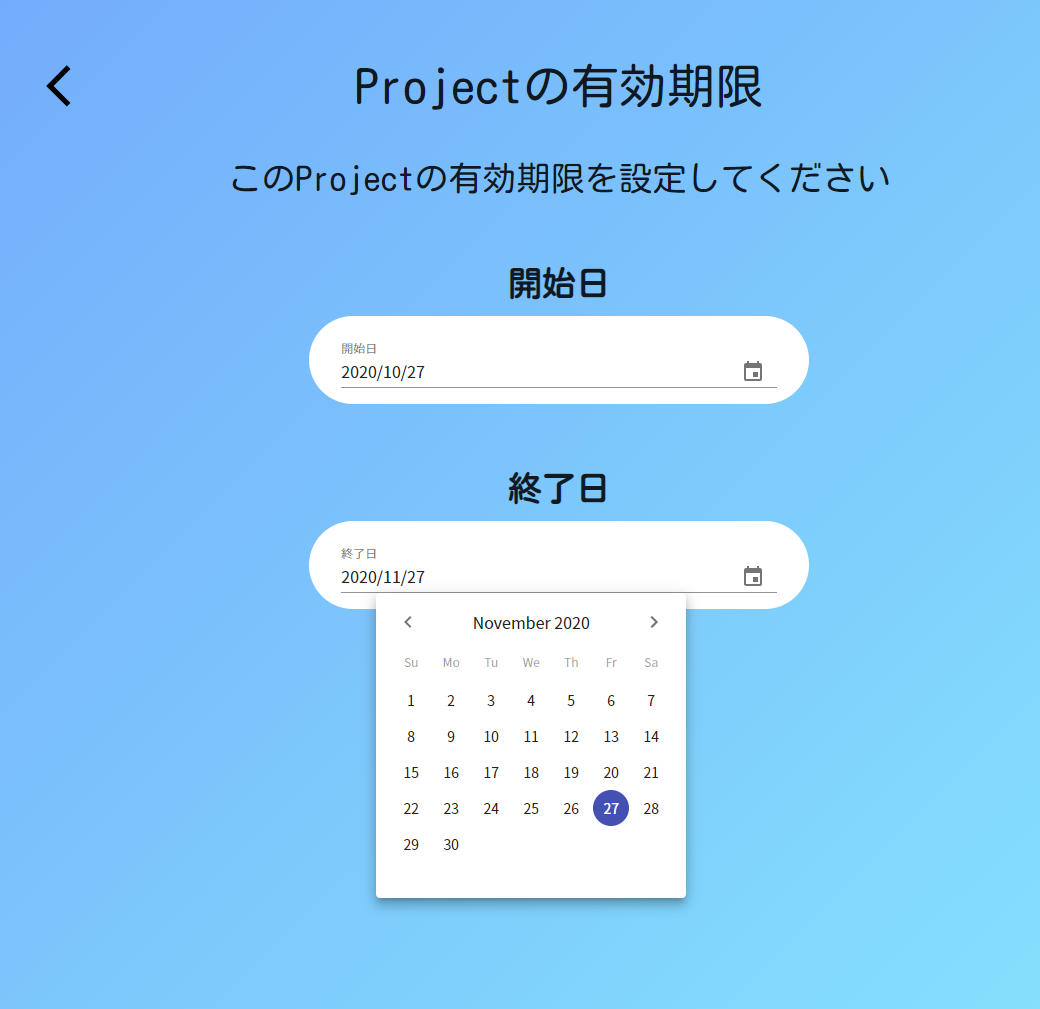
\includegraphics[width=100mm]{period.png}
  \caption{有効期限ページの入力画面と入力例}
  \label{period}
\end{figure}

有効期限ページ(図\ref{period})では,センシング開始日とセンシング終了日入力を行う.
この入力ページでは,どちらの入力項目も必須項目である.
入力フォームは,日付の入力を簡易化するためにカレンダーのポップアップからの入力を可能にする.
この2つの項目は,サーバに定義されたProjectモデルの「startDate」と「endDate」に対応している.
% (img sensors.png cap: センサ設定ページの入力画面と入力例)
\begin{figure}[H]
  \centering
  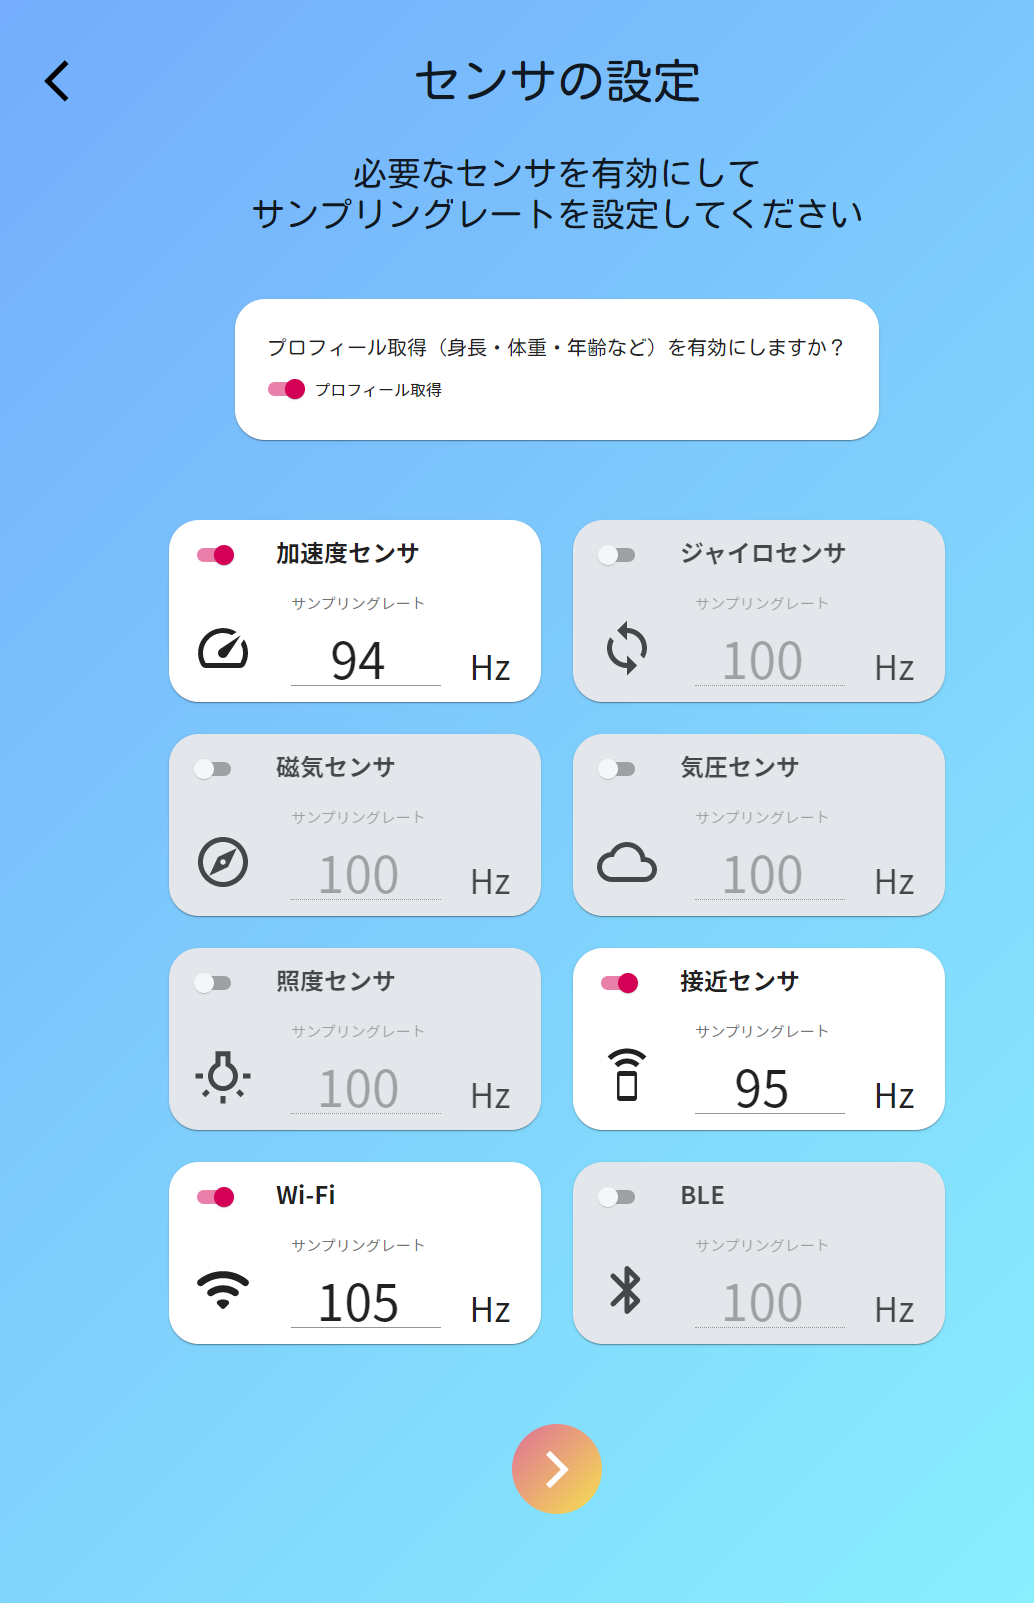
\includegraphics[width=100mm]{sensors.png}
  \caption{センサ設定ページの入力画面と入力例}
  \label{sensors}
\end{figure}

センサ設定ページ(図\ref{sensors})では,協力者に自身の基礎情報を求めるかの有無とセンサの設定を行う.
協力者に協力者の基礎情報を求める設定は,3.3.2項「センシングデータの管理や各プロジェクトを管理するサーバの実装」にも記述があるが,現在実装には至っていないため定義のみとなる.
この入力ページでは,一つ以上のセンサの設定が必須である.
このページのフォームの入力方法はトグルスイッチを採用しており,トグルスイッチにより有効になった設定と無効な設定を判別しやすいようにそれぞれの項目が明るくなるようになっている.
また,各センサの設定は文字だけでなくアイコンを用いてそれぞれのセンサの設定を視覚的に判別しやすいようにしており,トグルスイッチによりサンプリングレートの入力が有効化されサンプリングレートの設定を行う.
この2つの項目は,サーバに定義されたSensingSettingモデルの「isProvidedProfile」と「sensors」に対応している.
% (img areaInput.png cap: 時空間フェンシング設定ページのエリア入力画面と入力例)
\begin{figure}[H]
  \centering
  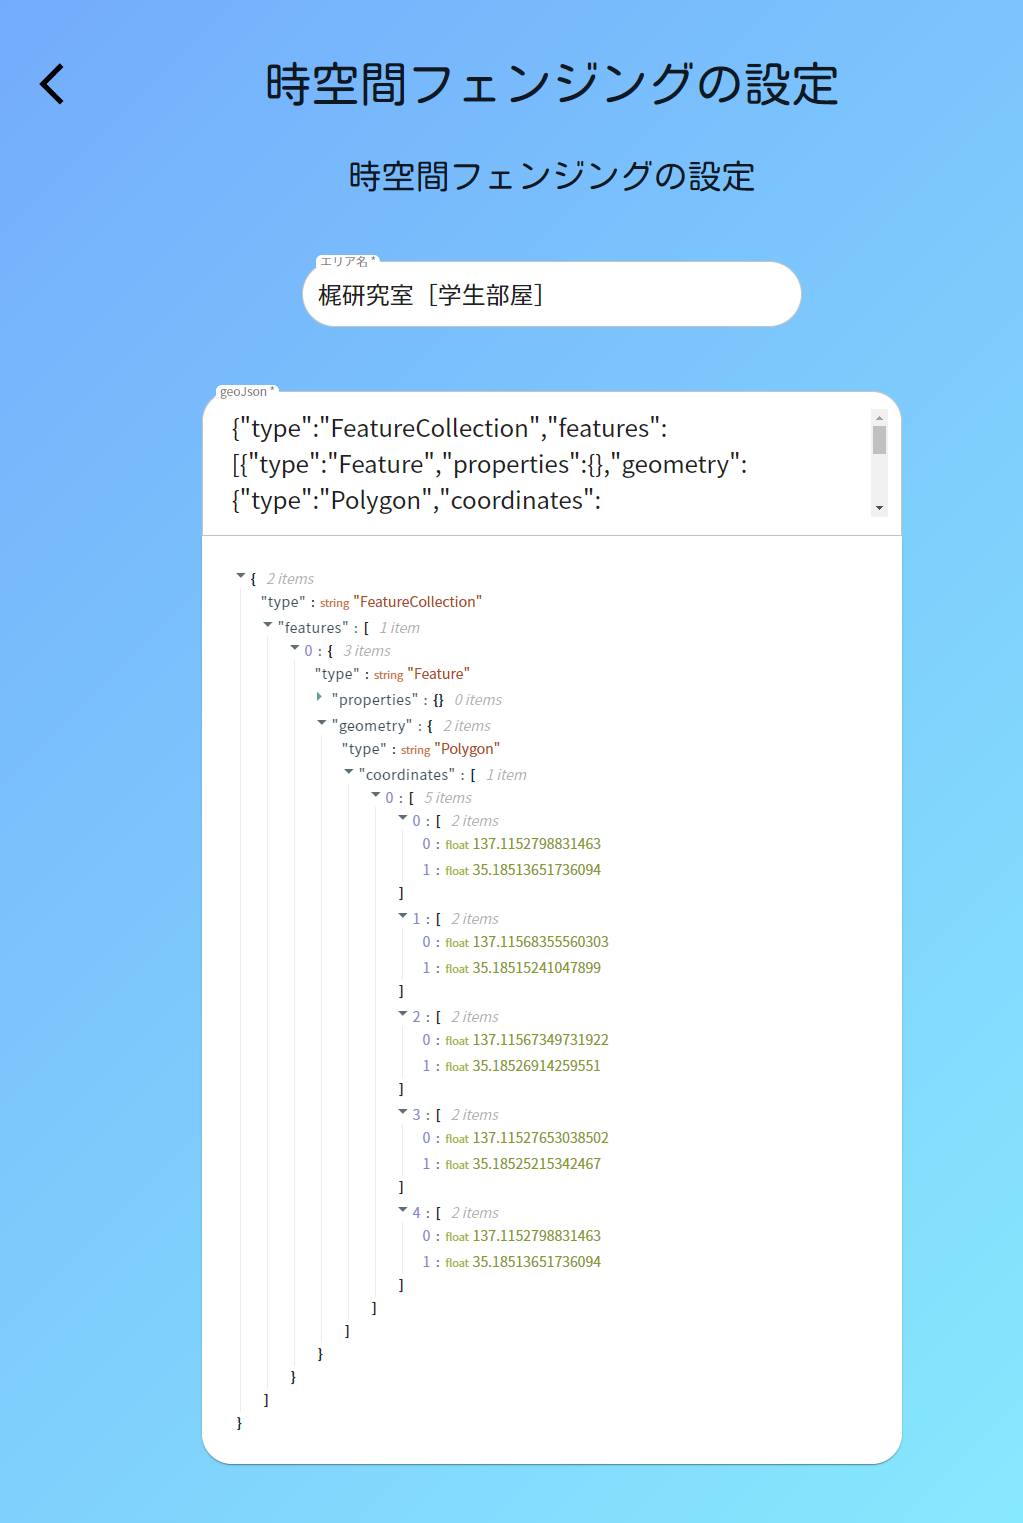
\includegraphics[width=120mm]{areaInput.png}
  \caption{時空間フェンシング設定ページのエリア入力画面と入力例}
  \label{areaInput}
\end{figure}

時空間フェンシング設定ページ(図\ref{areaInput})では,時空間フェンシングに必要なエリアの設定と時間帯の設定を行う.
この入力ページでは,エリア名の入力とエリア設定,時間帯を1つ以上の設定が必須である.
エリアの入力では,GeoJSON形式のテキストの入力を行う.
この入力フォームは,geojson.io\cite{geojson}等のサイトを用いてGeoJSON形式のテキストを取得・入力を前提としている.
図\ref{geojsonIo}は,geojson.ioを利用してGeoJSON形式のテキストを取得する例である.
% (img geojsonIo.png cap: geojson.ioを利用したGeoJSON形式のテキストの取得と入力例)
\begin{figure}[H]
  \centering
  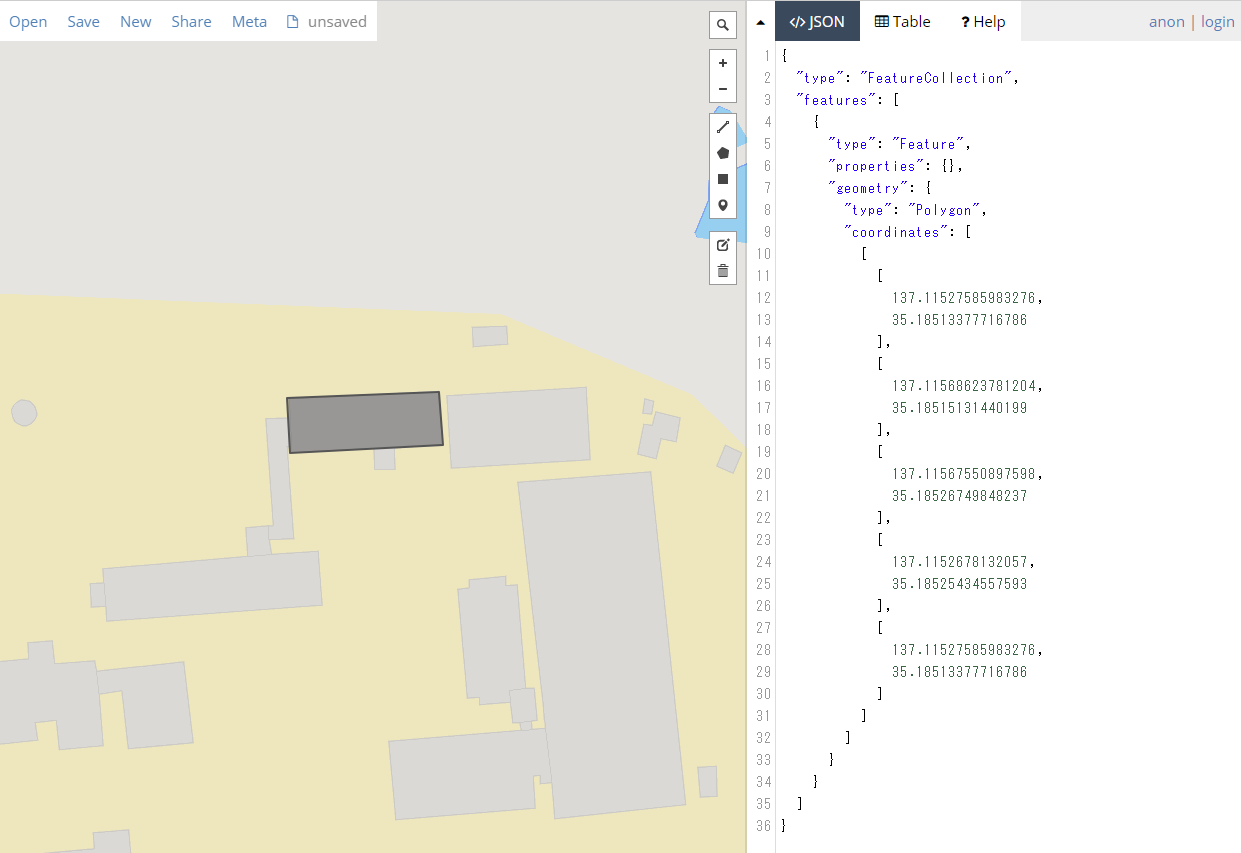
\includegraphics[width=150mm]{geojsonIo.png}
  \caption{geojson.ioを利用したGeoJSON形式のテキストの取得と入力例}
  \label{geojsonIo}
\end{figure}

% (img geojsonIo.png cap: エリア設定入力にGeoJSONでない形式のテキストを入力する例)
\begin{figure}[H]
  \centering
  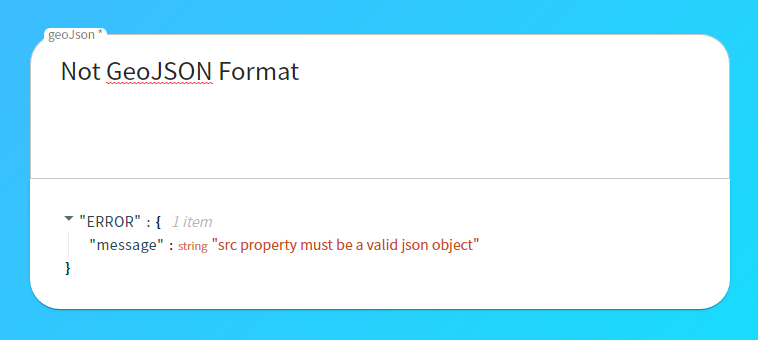
\includegraphics[width=120mm]{notGeoJSONFormat.png}
  \caption{エリア設定入力にGeoJSONでない形式のテキストを入力する例}
  \label{fig401}
\end{figure}

取得したGeoJSON形式のテキストを入力すると,入力フォームの下部に整形されたGeoJSONの情報の確認が可能である.
図\ref{fig401}のようにGeoJSON形式でない文字を入力すると,エラーが表示される様になっているため,入力が正常に行われているのかの確認が可能である.

% (img timeInput.png cap: 時空間フェンシング設定ページの時間帯入力画面と入力例)
\begin{figure}[H]
  \centering
  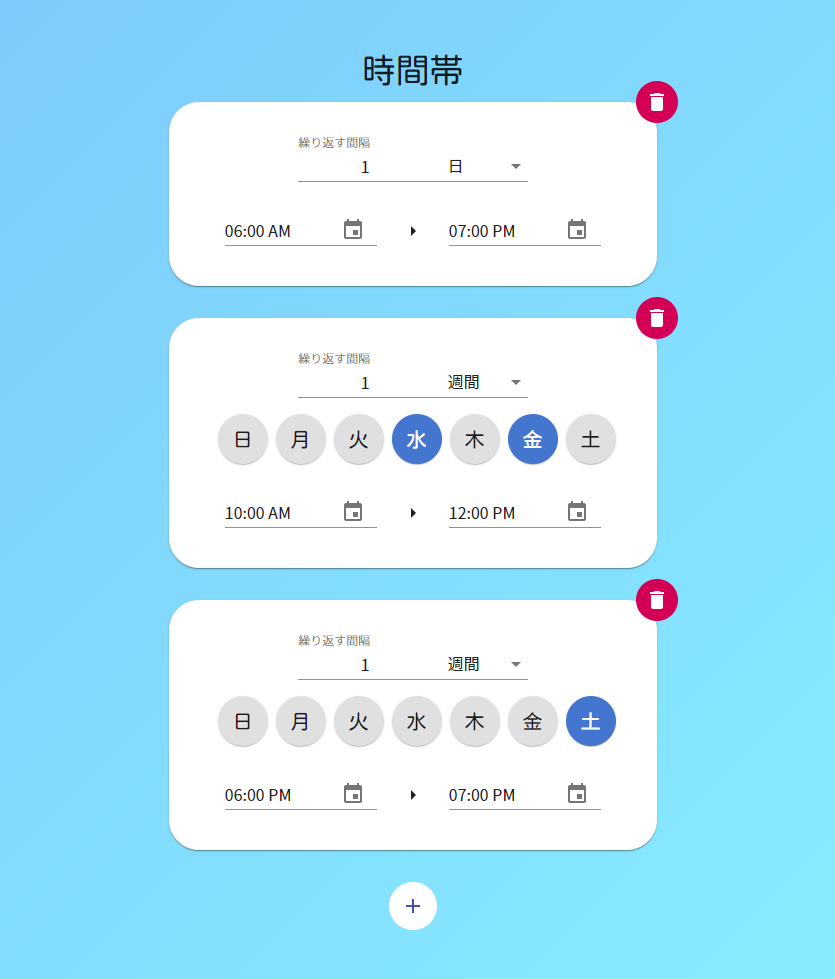
\includegraphics[width=120mm]{timeInput.png}
  \caption{時空間フェンシング設定ページの時間帯入力画面と入力例}
  \label{timeInput}
\end{figure}

% (img timeModal.png cap: 時間の入力モーダル)

\begin{figure}[H]
  \centering
  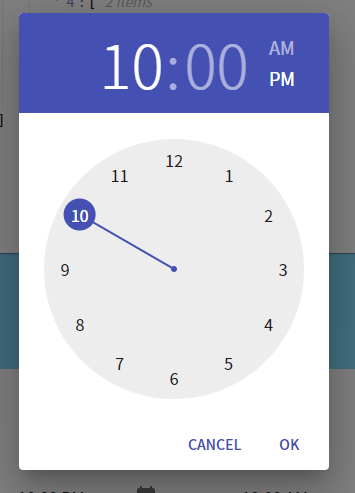
\includegraphics[width=50mm]{timeModal.png}
  \caption{時間の入力モーダル}
  \label{timeModal}
\end{figure}

時間帯の入力フォームでは,3.3.2項「センシングデータの管理や各プロジェクトを管理するサーバの実装」で定義した複数の時間帯を定義可能なフォーマットに対応した入力フォームを作成する.
このフォームは,繰り返す間隔の数字入力とその右側に単位の選択を行うセレクタがあり,セレクタでは「日」と「週間」のどちらかを選択する.
セレクタで「週間」を選択した場合のみ,その下部に曜日を示すボタンが表示され,ボタンをクリックし曜日の指定を行う.
最下部には開始時間と終了時間の入力項目があり,それぞれのフォームのクリックにより,図\ref{timeModal}のような時間を入力するモーダルが表示され時間の入力を行う.
複数の時間帯を定義する場合は,フォーム下部の+ボタンをクリックにより複数の時間帯を定義できる.
また,定義した時間帯の削除を行う場合はフォーム右上のゴミ箱のアイコンをクリックする.
この3つの項目は,サーバに定義されたSensingSettingモデルの「areaName」と「geo」と「periodOftimes」に対応している.
以上の項目をすべて入力後の送信ボタンクリックにより,サーバの「/project」及び「/sensing-setting」エンドポイントに入力情報が送信される.
センシングプロジェクトの定義が完了となり開始日になると,センシングプロジェクトが開始される.

\begin{figure}[H]
  \centering
  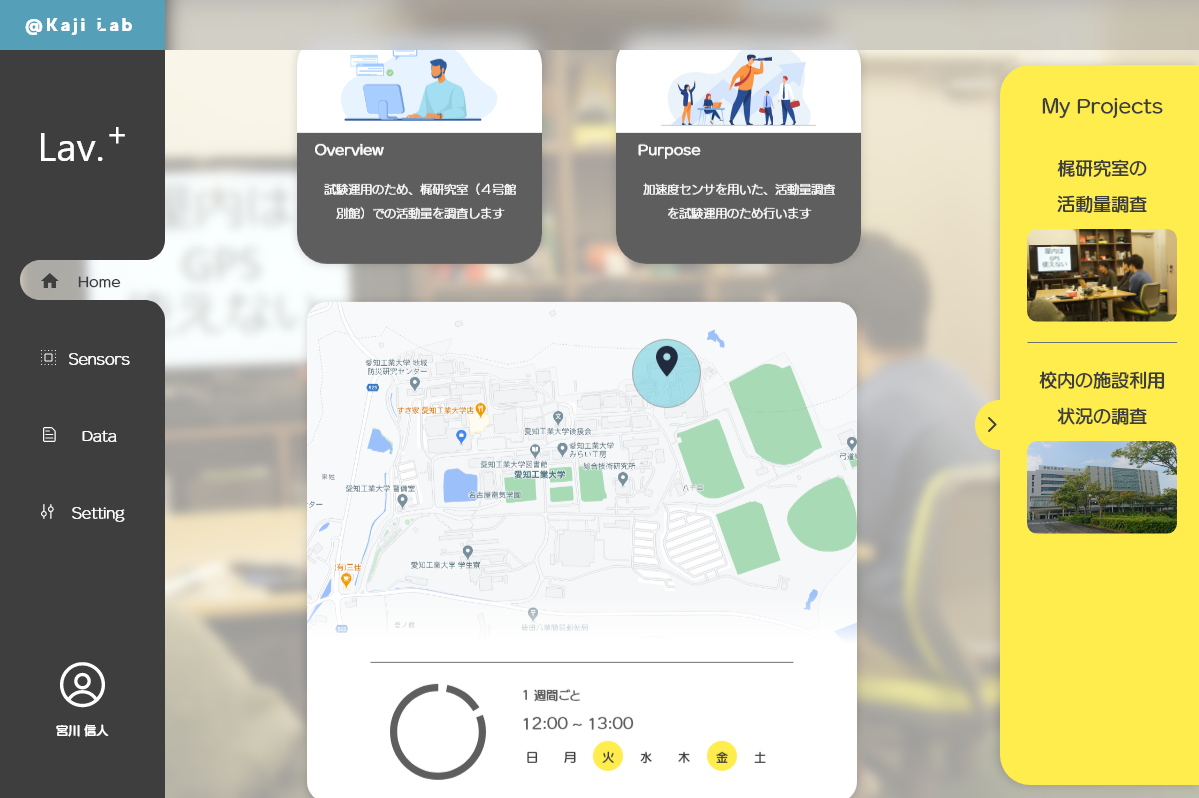
\includegraphics[width= 150mm]{Dashboard.png}
  \caption{管理画面ページ}
  \label{server}
\end{figure}

センシングプロジェクトの定義を終了すると,管理画面にて定義したセンシングプロジェクトの情報閲覧が可能となる.
協力者からセンシングデータを提供されると,その管理画面よりそのセンシングデータのダウンロードが可能となる.
ラヴラスでは依頼者1人による複数のプロジェクトの作成を想定し,管理画面の右側に表示されたメニューより作成したセンシングプロジェクトの切り替え及び追加作成が可能となっている.

\begin{figure}[H]
  \centering
  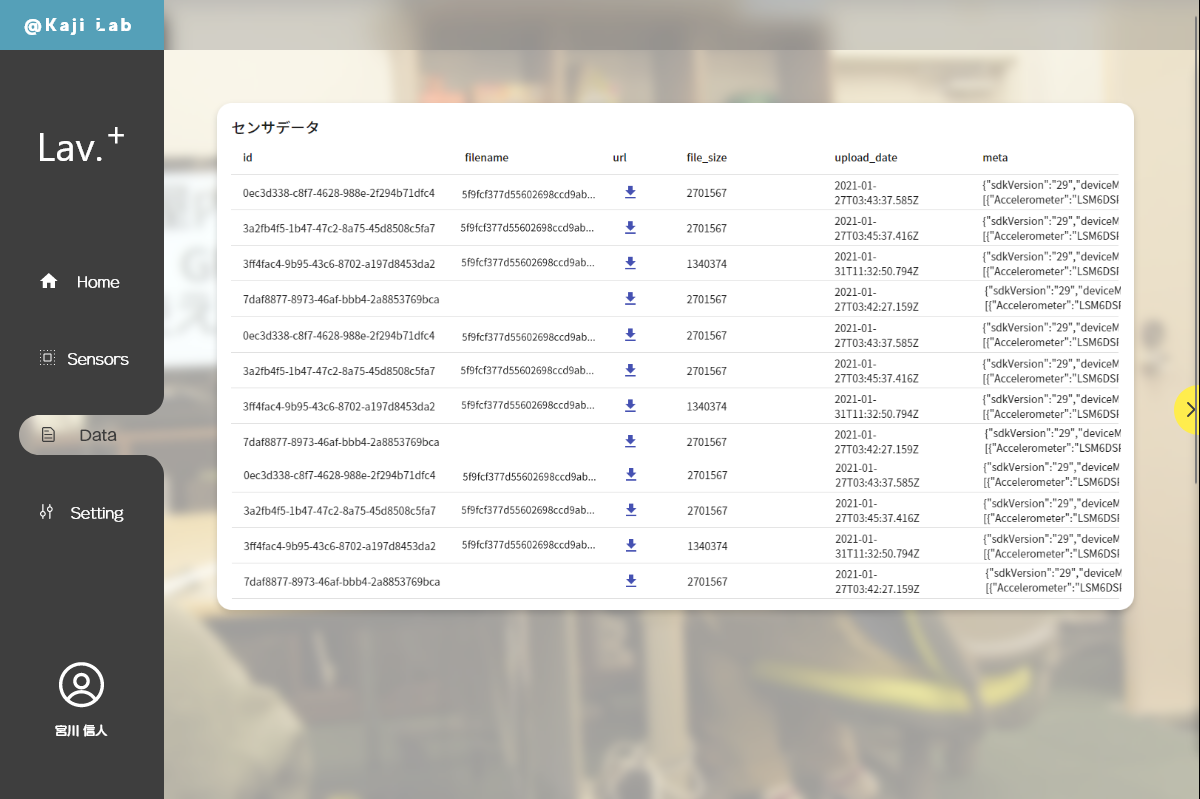
\includegraphics[width= 150mm]{Dashboard-SensingData.png}
  \caption{提供されたセンシングデータの一覧及びダウンロードを行うページ}
  \label{server}
\end{figure}

提供されたセンシングデータのダウンロードは,Dataメニューのクリックによりセンシングデータの一覧が表示され,ファイル名,ファイルサイズ,アップロード日,メタデータの情報を確認できる.
センシングデータのダウンロードは,一覧の各列のダウンロードボタンのクリックにより可能である.
% -----------------------------------------------

\subsection{協力者用のセンシングスマホアプリの実装}

\begin{figure}[H]
  \centering
  \includegraphics[width= 150mm]{serverApp.png}
  \caption{サーバとスマホアプリの連携}
  \label{server}
\end{figure}


ラヴラスでは,協力者がセンシングプロジェクト毎にスマホアプリをインストールする手間を省くため,協力者専用のAndroidアプリケーションを作成する.
第1章でも述べたように,スマートフォンの利用者は使用頻度の低いアプリケーションを削除する傾向にある.
理由としては,ストレージの容量確保のためであったり,整理整頓であったりと様々である.
例えば,本プラットフォームのような基盤を用いず,個別の専用アプリケーションを作成し,クラウドセンシングを行うとする.
この場合,専用アプリケーションの数は研究の数と比例する.
クラウドセンシングを利用して行いたい人が増えれば増えるほど,個別の専用アプリケーションも増えていく.
その都度協力者はアプリケーションをインストールする必要がある.
インストールには時間や手間がかかり,ストレージを使用してしまう.
1回ならまだしも,インストールの回数が2回3回と増えていくと,クラウドセンシング自体が面倒になり,非協力的になってしまう可能性がある.
ストレージの使用容量が微量だったとしても,空き容量がなくなった場合に真っ先に削除される可能性もある.
依頼者が別のクラウドセンシングを行う際,前回のシステムをそのまま使うとしても,アップデートや再インストールが必要となるため,協力者にとっては負担になる.
また,一定期間クラウドセンシングを行わなかった場合,協力者は「もうこのアプリケーションでのセンシングは終わったのだ」と解釈し,削除する可能性がある.
こうなると,いざもう一度センシングを行おうとなったときに協力者がいるとは限らない.
個別でクラウドセンシングアプリケーションを作成する問題点として,仕様や操作法の違いも挙げられる.
クラウドセンシングは一定の基準が定められている訳ではないため,依頼者独自の仕様や操作法である.
アプリ毎に仕様を理解し操作するのは協力者にとって大きな負担になる.
依頼者が所属している研究室の教授であったり,友人である場合,そのような負担も気にならないかもしれないが,赤の他人であった場合,
協力者が本スマホアプリをインストールすれば,本プラットフォームで作成されたセンシングプロジェクトに協力が可能となる.
これにより,依頼者はクラウドセンシングを利用するために,一からセンシング専用のスマホアプリを開発する必要がなくなり,協力者はクラウドセンシングに協力するために,何度もインストールする必要がなくなる.

本スマホアプリはサーバと連携し,センシングプロジェクトの受信やセンシングデータファイルとメタデータのアップロードを行う.
センシングプロジェクトは適宜サーバから取得し,本スマホアプリ内のデータベースに登録する.
新規のセンシングプロジェクトの場合は新しく登録し,既存のセンシングプロジェクトの場合は内容が変更している可能性を考慮して最新の方に更新する.
データベースより現在時刻から一番近い指定開始時間を検索し,指定開始時間と指定終了時間を時空間フェンシングに設定する.
また,設定した時間と同じセンシングプロジェクトのエリアとプロジェクトIDも設定しておく.
プロジェクトIDは時空間内に進入した際に送られる通知画面に表示されるプロジェクト内容の検索に用いる.

時空間フェンシングは位置情報取得を最小限にするために,まず時間判定を行い,センシングプロジェクトで指定された開始時間にエリア判定を行う.
時間判定とエリア判定を平行して行った場合でも,問題なく時空間フェンシングは動作する.
しかし,我々のクラウドセンシングの中枢として,協力者の負担軽減がある.
位置情報の収集とスマートフォンの電池の消耗は直接的な関係がある.
例えば,位置情報データの精度が高ければ高いほど電池の消耗は激しくなる.
また,位置情報の計算頻度が高ければ高いほど電池の消費量は増加する.
つまり,位置情報の精度と計算頻度が高いほど,より多くの電池量を消費するのである.
そのため,スマートフォンの負担を軽減するには,低い精度と計算頻度で妥協する必要がある.
しかし,時空間フェンシングを行う上で,位置情報は非常に重要な情報である.
位置情報の精度が低いと,実際にはエリア内に進入しているのにスマートフォン上ではエリア外となってしまったり,反対にエリア外にいるのにエリア内に進入しているとなってしまう可能性がある.
それにより,途中でセンシングが終了してしまったり,ずっとエリア内にいるのにセンシング依頼通知が送られてないなどセンシングに支障をきたしてしまう.
よって,位置情報の精度の低減もできない.
指定開始時間以前に指定エリア内に入っていてもセンシングは開始しないし,スマートフォンの充電を無駄に消耗させてしまう.
そのため,指定開始時間後にエリア判定を行う.

協力者が指定センシングエリア内に進入したか否かは,点の多角形に対する内外判定\cite{naigai}で判定する.
点の多角形に対する内外判定を図\ref{naigaihantei}に示す.
点の内外判定とは,まず点(赤丸)から多角形に対して水平線を引く.
その線と多角形との交点(青丸)の数が奇数個であれば多角形よりも内側にいる,偶数個であれば多角形よりも外側にいると判定できる.
この場合,丁度線と多角形の辺が重なったり,線と多角形の頂点と重なると,誤った判定を行ってしまう.
しかし,緯度経度は小数点以下が7桁もあり,位置情報は変化し続けるため,丁度重なる場合は今回考えないものとしている.
実装当初は内外判定ではなく条件分岐を用いて,エリア判定を行っていた.
現在位置の緯度が指定エリアの最北端よりも低く最南端よりも高い,また経度が指定エリアの最東端よりも低く最西端よりも高い場合,指定エリア内にいると判定した.
しかし,この条件分岐を用いると,自ずと判定範囲が矩形になってしまう.
そうなった場合,正常にエリア判定できるのは緯度経度と平行な矩形のみとなる.
例えば,指定センシングエリアがひし形の場合を想定する.
正常なエリア判定としては,図\ref{risou}の通り現在地(赤丸)にいた場合はエリア内に進入していないため,通知は送られないはずである.
しかし,条件分岐を用いたエリア判定の場合は,ひし形の外側にひし形の頂点を辺の中心とした矩形の判定エリアが形成されるため,図\ref{bunki}のように現在地がエリア内にいると判定され,誤って通知が送られてしまう.
一方で,点の内外判定は現在地から水平に引いた線とひし形のエリアの交点(青丸)が2つと偶数個であるため,エリア外と判定できる(図\ref{orr}).
これにより,依頼者が図\ref{naigaihantei}のようにどれだけ複雑な多角形のエリアを設定しても,内部か否かは判定可能である.
今回は実装は行っていないが円のようなエリアでも判定は可能である.
また,今回はGPSのみを用いたエリア判定のため,平面的なエリア判定しか行えない.
1階や2階などの立体的なエリア判定は今後の課題とする.

\begin{figure}[H]
    \begin{center}
      \begin{tabular}{c}
  
        % 1
        \begin{minipage}{0.5\hsize}
            \begin{center}
            
            \begin{tikzpicture}
   
                
                \coordinate  (A) at (1,1); %点A
                \coordinate  (B) at (5,1); %点B
                \coordinate  (C) at (4,2); %点C
                \coordinate  (D) at (4,4); %点D
                \coordinate  (E) at (1,4); %点D
                \coordinate  (F) at (1,2); %点D
                \coordinate  (J) at (2,2); %点D
                \coordinate  (K) at (2,3); %点D
                \coordinate  (G) at (3,3); %点D
                \coordinate  (H) at (3,2); %点D
                \coordinate  (I) at (3,1.5); %点D
                \coordinate  (L) at (1.5,2.5); %点D
                \coordinate  (M) at (4.5,1.5); %点D
                \coordinate  (N) at (2,2.5); %点D
                \coordinate  (O) at (3,2.5); %点D
                \coordinate  (P) at (4,2.5); %点D
                % \coordinate [label=現在地](E) at (0.5,1.5); %点E
                \foreach \P in {A,B,C,D,E,F,G,J,K,H} \fill[black] (\P) circle (0.08);  %点A,B,Cに黒丸
                
                \foreach \P in {I,L} \fill[red] (\P) circle (0.08);
                \draw (A) -- (B) -- (C) -- (D) -- (E) -- (F) -- (J) -- (K)-- (G) -- (H) -- cycle;
                % \draw (0,0) -- (3,0) -- (0,1) -- cycle;
                % \draw (3,0) -- (6,0) -- (6,1) -- cycle;
                % \draw (6,1) -- (6,2) -- (3,2) -- cycle;
                % % \draw (0,1) -- (0,2) -- (3,2) -- cycle;
                % \fill[lightgray] (A) -- (B) -- (C) -- (D) -- cycle;
                \draw[->,>=stealth,semithick] (3,1.5)--(7,1.5)node[above]{$交点1つ$};
                \draw[->,>=stealth,semithick] (1.5,2.5)--(7,2.5)node[above]{$交点3つ$};
                \foreach \P in {M,N,O,P} \fill[cyan] (\P) circle (0.08);
        
            \end{tikzpicture}
            \hspace{1.9cm} 点が多角形より内側の場合は交点が奇数個


        \end{center}
        \end{minipage}

        % 1
        \begin{minipage}{0.5\hsize}
            \begin{center}
            
            \begin{tikzpicture}
   
                
                \coordinate  (A) at (1,1); %点A
                \coordinate  (B) at (5,1); %点B
                \coordinate  (C) at (4,2); %点C
                \coordinate  (D) at (4,4); %点D
                \coordinate  (E) at (1,4); %点D
                \coordinate  (F) at (1,2); %点D
                \coordinate  (J) at (2,2); %点D
                \coordinate  (K) at (2,3); %点D
                \coordinate  (G) at (3,3); %点D
                \coordinate  (H) at (3,2); %点D
                \coordinate  (I) at (1,1.5); %点D
                \coordinate  (L) at (2.5,2.5); %点D
                \coordinate  (M) at (4.5,1.5); %点D
                \coordinate  (N) at (2,1.5); %点D
                \coordinate  (O) at (3,2.5); %点D
                \coordinate  (P) at (4,2.5); %点D
                % \coordinate [label=現在地](E) at (0.5,1.5); %点E
                \foreach \P in {A,B,C,D,E,F,G,J,K,H} \fill[black] (\P) circle (0.08);  %点A,B,Cに黒丸
                
                \foreach \P in {I,L} \fill[red] (\P) circle (0.08);
                \draw (A) -- (B) -- (C) -- (D) -- (E) -- (F) -- (J) -- (K)-- (G) -- (H) -- cycle;
                % \draw (0,0) -- (3,0) -- (0,1) -- cycle;
                % \draw (3,0) -- (6,0) -- (6,1) -- cycle;
                % \draw (6,1) -- (6,2) -- (3,2) -- cycle;
                % % \draw (0,1) -- (0,2) -- (3,2) -- cycle;
                % \fill[lightgray] (A) -- (B) -- (C) -- (D) -- cycle;
                \draw[->,>=stealth,semithick] (1,1.5)--(6.5,1.5)node[above]{$交点2つ$};
                \draw[->,>=stealth,semithick] (2.5,2.5)--(7,2.5)node[above]{$交点2つ$};
               \foreach \P in {M,N,O,P} \fill[cyan] (\P) circle (0.08);
               
            \end{tikzpicture}
            \hspace{1.6cm} 点が多角形より外側の場合は交点が偶数個
        \end{center}
        \end{minipage}
  
        
  
      \end{tabular}
      
      
      \caption{点の多角形に対する内外判定}
      \label{naigaihantei}
    \end{center}
  \end{figure}

\begin{figure}[H]
    \begin{center}
      \begin{tabular}{c}
  
        % 1
        \begin{minipage}{0.5\hsize}
            \begin{center}
            
            \begin{tikzpicture}
   
                \draw[->,>=stealth,semithick] (-0.1,0)--(6.5,0)node[above]{$lng$}; %x軸
                \draw[->,>=stealth,semithick] (0,-0.1)--(0,2.5)node[right]{$lat$}; %y軸
                \draw (0,0); %原点
 
                \coordinate  (A) at (0,1); %点A
                \coordinate  (B) at (3,0); %点B
                \coordinate  (C) at (6,1); %点C
                \coordinate  (D) at (3,2); %点D
                \coordinate [label=現在地](E) at (0.5,1.5); %点E
                \foreach \P in {A,B,C,D} \fill[black] (\P) circle (0.08);  %点A,B,Cに黒丸
                \foreach \P in {E} \fill[red] (\P) circle (0.08);
                 \draw (A) -- (B) -- (C) -- (D) -- cycle;
                % \draw (0,0) -- (3,0) -- (0,1) -- cycle;
                % \draw (3,0) -- (6,0) -- (6,1) -- cycle;
                % \draw (6,1) -- (6,2) -- (3,2) -- cycle;
                % \draw (0,1) -- (0,2) -- (3,2) -- cycle;
                \fill[lightgray] (A) -- (B) -- (C) -- (D) -- cycle;

        
            \end{tikzpicture}
            \hspace{1.6cm} 現在地→エリア外\\エリア判定上→エリア外
            \caption{正常なエリア判定}
            \label{risou}
        \end{center}
        \end{minipage}
  
        % 2
        \begin{minipage}{0.5\hsize}
          \begin{center}
            \begin{tikzpicture}
   
                \draw[->,>=stealth,semithick] (-0.1,0)--(6.5,0)node[above]{$lng$}; %x軸
                \draw[->,>=stealth,semithick] (0,-0.1)--(0,2.5)node[right]{$lat$}; %y軸
                \draw (0,0); %原点
                \coordinate (A) at (0,1); %点A
                \coordinate (B) at (3,0); %点B
                \coordinate (C) at (6,1); %点C
                \coordinate (D) at (3,2); %点D
                \foreach \P in {A,B,C,D} \fill[black] (\P) circle (0.08);  %点A,B,Cに黒丸
                
                \draw (A) -- (B) -- (C) -- (D) -- cycle;
                \draw (0,0) -- (3,0) -- (0,1) -- cycle;
                \draw (3,0) -- (6,0) -- (6,1) -- cycle;
                \draw (6,1) -- (6,2) -- (3,2) -- cycle;
                \draw (0,1) -- (0,2) -- (3,2) -- cycle;
                \fill[lightgray] (0,0) -- (3,0) -- (0,1) -- cycle;
                \fill[lightgray] (3,0) -- (6,0) -- (6,1) -- cycle;
                \fill[lightgray] (6,1) -- (6,2) -- (3,2) -- cycle;
                \fill[lightgray] (0,1) -- (0,2) -- (3,2) -- cycle;
                \fill[lightgray] (A) -- (B) -- (C) -- (D) -- cycle;
                \coordinate [label=現在地](E) at (0.5,1.5); %点E
                \foreach \P in {E} \fill[red] (\P) circle (0.08);
        
            \end{tikzpicture}
            \hspace{1.6cm} 現在地→エリア外\\エリア判定上→エリア内
            \caption{条件分岐による矩形でのエリア判定}
            \label{bunki}
          \end{center}
        \end{minipage}
  
      \end{tabular}
      
      \label{fig:lena}
    \end{center}
  \end{figure}

  \begin{figure}[H]
    \begin{center}
      \begin{tabular}{c}
  
        % 1
        \begin{minipage}{0.5\hsize}
            \begin{center}
            
            \begin{tikzpicture}
   
                \draw[->,>=stealth,semithick] (-0.1,0)--(6.5,0)node[above]{$lng$}; %x軸
                \draw[->,>=stealth,semithick] (0,-0.1)--(0,2.5)node[right]{$lat$}; %y軸
                \draw (0,0); %原点
 
                \coordinate  (A) at (0,1); %点A
                \coordinate  (B) at (3,0); %点B
                \coordinate  (C) at (6,1); %点C
                \coordinate  (D) at (3,2); %点D
                \coordinate  (F) at (1.5,1.5); %点D
                \coordinate  (G) at (4.5,1.5); %点D
                \coordinate [label=現在地](E) at (0.5,1.5); %点E
                \foreach \P in {A,B,C,D,F,G} \fill[black] (\P) circle (0.08);  %点A,B,Cに黒丸
                
                \foreach \P in {E} \fill[red] (\P) circle (0.08);
                 \draw (A) -- (B) -- (C) -- (D) -- cycle;
                % \draw (0,0) -- (3,0) -- (0,1) -- cycle;
                % \draw (3,0) -- (6,0) -- (6,1) -- cycle;
                % \draw (6,1) -- (6,2) -- (3,2) -- cycle;
                % % \draw (0,1) -- (0,2) -- (3,2) -- cycle;
                % \fill[lightgray] (A) -- (B) -- (C) -- (D) -- cycle;
                \draw[->,>=stealth,semithick] (0.5,1.5)--(6.5,1.5);
                \foreach \P in {F,G} \fill[cyan] (\P) circle (0.08);
        
            \end{tikzpicture}
            \hspace{1.6cm} 線とエリアの交点が2つ→エリア外
        \end{center}
        \end{minipage}
  
        
  
      \end{tabular}
      \caption{点の内外判定でのエリア判定}
      \label{orr}
    \end{center}
  \end{figure}

% 本アプリケーションが取得する位置情報は常に正確であるとは限らないため,marginを用いて進入時にはエリアを縮小,退出時には拡大する.

協力者がセンシングプロジェクトで指定された時間帯とエリア内に進入したら,通知を送る.
通知はヘッドアップ通知で,振動ありで送られる.
ヘッドアップ通知により,スマートフォンを使用している際に目に留まりやすく,また振動もあるため,スマートフォンの画面を見ていない時やポケットに入れている時により気がつきやすくなる.
通知のタップにより,アプリケーションを開き,センシング依頼の通知画面が表示される.
通知画面では現在地と指定エリアをGoogle Mapsで,時間帯をバーで,センシングプロジェクトの内容をスクロールで表示し,協力者に確認してもらう.
指定エリアのマップ表示により,テキストよりも指定エリアの広さが解りやすく,現在地との位置関係も把握しやすい.


% センサの処理やセンシングデータファイルの作成などセンシングの大部分は,HASC Loggerという行動センシングデータを収集するアプリケーションの仕組みを参考に実装した.

% サーバとのHTTP通信では,センシングプロジェクトの取得やセンシングデータファイルのアップロードなどを行う.

センシングデータファイルはディレクトリを監視し,ファイルへのセンシングデータ書き込み終了(書き込み用にファイルを開いて閉じた)を判定したとき,協力者のスマートフォンがWi-Fiに接続されていればアップロードされる.
まず協力者が指定エリアから退出した及び指定終了時間になった時,実行中のセンシングを終了する.
センシング終了後,センシングデータを書き込んでいたファイルを閉じた際にイベント判定を行い,ファイルアップロードの段階に入る.
ファイルアップロードでは,まずデータベースにセンシングファイル名とファイルを未アップロードという情報を紐づけて登録する.
次に,Wi-Fiなどのインターネット接続の有無を確認し,接続されている場合のみアップロードを行い,未アップロードの情報を更新する.
携帯回線に接続された状態でセンシングデータをアップロードしてしまうと,協力者のモバイル通信量を使用し負担をかけてしまう.
手動でデータアップロードする場合は,携帯回線を好まない場合にWi-Fiに接続できる場所に移動してからアップロードするなど判断ができるため,アプリケーション側の配慮は必要としない.
しかし,自動でアップロードする場合,判断する余地がないため,負担の少ないWi-Fiに接続時のみにしなければならない.
もし,Wi-Fiに接続されていない場合は,アップロードを見送り,次回ファイルアップロードの段階に入った際にまとめてアップロードする.

協力者の操作を最小限にするため,時空間フェンシングやセンシング,センシングデータのアップロードなどアプリの大部分はバックグラウンドで行う.
そのため,スマホアプリを意識して開く必要はない.
開くのは時空間内に進入した際に送られるヘッドアップ通知をタップした時のみである.
それ以外は基本的に画面上のアイコンをタップしてアプリケーションを開くなどは不要である.
通知画面を承諾した後も,「センシング中はアプリケーションを開いておかなければならない」という仕様ではないため,すぐに閉じても構わない.
アプリケーション自体を終了させなければ,途中でセンシングは終了しない.
バックグラウンドにより,協力者の操作などの負担の軽減に加え,センシングをしているという感覚を意識させないため,より普段の振る舞いをセンシングできる.
% -----------------------------------------------

\section{動作検証}
本センシングプラットフォームを用いて,依頼者側のセンシングプロジェクトの作成やセンシングデータのダウンロード,協力者側の時空間フェンシングや通知,センシングプロジェクトに基づいたセンシング,センシングデータのアップロードなど一連の流れが正常に動作するか検証する.
動作が正常か否かを確認するためにチェック項目を設けた.
依頼者側のチェック項目としては,「センシングプロジェクトを作成できるか」,「アップロードされたセンシングデータはダウンロード可能か」を挙げた.
協力者側のチェック項目としては,「サーバからセンシングプロジェクトを受信できるか」「依頼者によって作成されたセンシングプロジェクトに基づいて,時空間フェンシングができているか」,「指定された時空間内に進入した際にヘッドアップ通知を送っているか」,「正しくセンシングできているか」,「センシング後,Wi-Fi接続時にセンシングデータをアップロードできているか」を挙げた.

\begin{figure}[H]
  \centering
  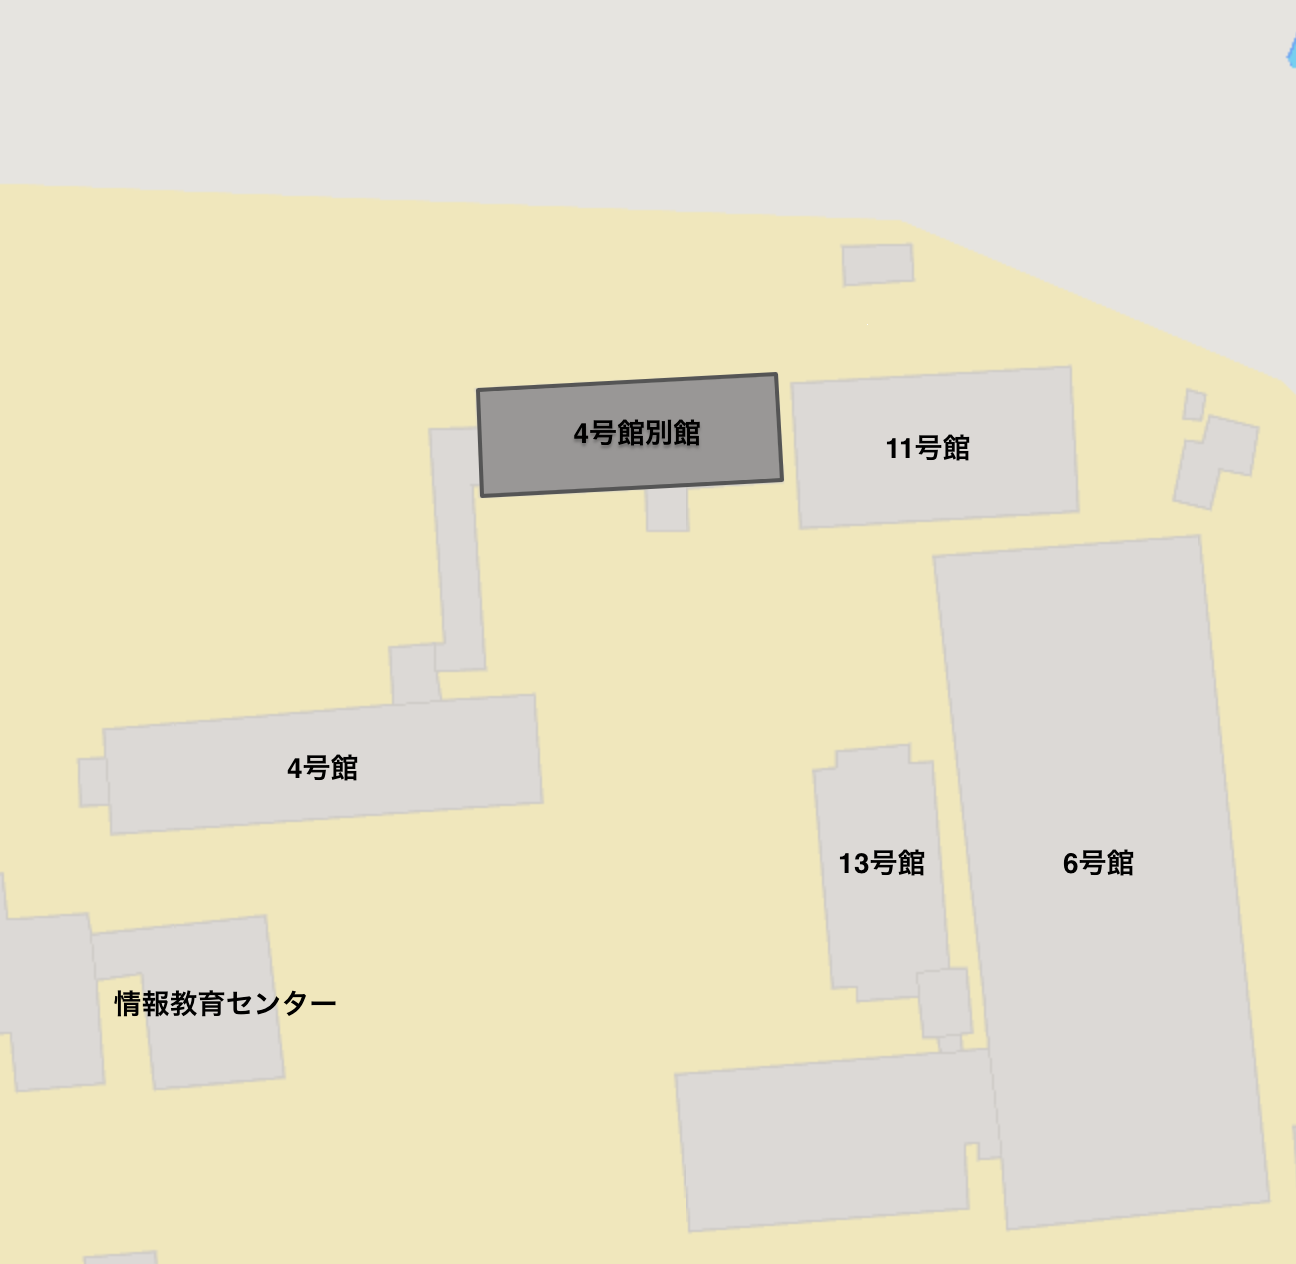
\includegraphics[width=100mm]{VerificationArea.png}
  \caption{動作検証エリア}
  \label{VerificationArea}
\end{figure}

今回の動作検証は,13時から14時までの愛知工業大学4号館別館(図\ref{VerificationArea})での活動量を加速度センサで調査するといったシナリオに基づいて行った.
スマートフォンはGoogle Pixel 4を使用した.
なお,今回の動作検証は実装の初期段階であるため,複雑な状況は想定せず,単純な状況で行う.
依頼者側は新規にWebアプリのユーザ登録を行い,協力者側は新規にスマホアプリをインストールする.
そのため,サーバには1つもセンシングプロジェクトがない状態とする.

結果として,我々が期待した通りの動作が確認できた.
まず,依頼者はWebアプリのユーザ登録を行う.

次に,Webアプリにてセンシングプロジェクトを作成する.
内容としては,時間帯を

協力者側のスマホアプリではサーバからセンシングプロジェクトを受信する.
サーバに定義された1つのセンシングプロジェクトを問題なく受信できたため,正常であると判断する.
次に,受信したセンシングプロジェクトに基づいて時空間フェンシングを行う.
指定開始時間(13時)前に動作検証エリアに進入しても通知は送られてこなかったが,指定開始時間になると通知が送られてきた.
エリアを退出するとセンシングは終了し,再度進入すると再度センシングが開始された.
エリアに進入したまま指定終了時間を迎えると,センシングは終了した.
これにより,時間判定・エリア判定ともに正常であると判断する.
動作検証エリアが屋内であるため,GPSでエリア判定を行うと位置情報誤差はあったが,動作は確認できた.屋内でのエリア判定は今後の課題とする.
また,通知も正常に送られていると確認できた.
次に,Wi-Fi接続時のみセンシングデータをアップロードする.
最初のセンシングはWi-Fiに接続していないモバイル通信の状態で終了した.
終了後にサーバを確認したところ,センシングデータは1件もなかった.
指定時間内に再度エリアに進入し,今回はWi-Fiに接続した状態でセンシングを終了した.
すると,サーバには今回のセンシングデータと最初のセンシング終了後にアップロードされなかったセンシングデータの2件が見受けられた.
Wi-Fiに接続時のみセンシングデータのアップロードは正常に確認できた.
動作検証エリアが屋内であるため,GPSでエリア判定を行うと位置情報誤差はあったが,動作は確認できた.屋内でのエリア判定は今後の課題とする.
指定した時空間内に進入すると,ヘッドアップ通知が表示され,それをタップし,依頼を承認するとセンシングが開始され,正常な動作が確認できた.
センシング後にサーバにアップロードされたセンシングデータを確認したところ,シナリオ通りに加速度が収集されていたため,動作検証は成功とする.

\begin{figure}[H]
  \centering
  \includegraphics[width=100mm]{sensingData.png}
  \caption{収集した生センシングデータ(一部)}
  \label{fig:2}
\end{figure}

% Local Variables: 
% mode: japanese-LaTeX
% TeX-master: "root"
% End: 


\chapter{特定の時空間への進入時に自動センシングするアプリケーション}
\thispagestyle{myheadings}
本章では特定の時空間への進入時に自動センシングするアプリケーションについて述べる.
\ref{lavlusReq}章ではまずラヴラスのモバイルアプリケーションの要求仕様を定義する.
\ref{myApp}章では特定の時空間への進入時に自動センシングするアプリケーションの実装に述べる.
\ref{myApp_STF}章では時空間フェンシングの実装について述べる.
\ref{myApp_notify}章ではセンシング依頼通知の実装について述べる.
\ref{myApp_sensing}章では自動センシングの実装について述べる.


\section{ラヴラスのモバイルアプリケーションの要求仕様}
\label{lavlusReq}
ラヴラスのモバイルアプリはセンシングプロジェクトダウンロード,時空間フェンシング,センシング依頼の承諾,自動的にセンシング,Wi-Fi環境下で自動的にアップロードができる必要がある.
協力者の物理的コストを軽減させるために,協力者への通知と協力者自身の操作の低減や,端末のデータ通信量を圧迫しない必要がある.
センシングプロジェクトをダウンロードする時,端末の通信量とデータ容量を圧迫しない為に,協力者が参加する可能性があるセンシングプロジェクトのみダウンロードする必要がある.
また,センシングが終わった後,Wi-Fiに接続している時に自動でアップロードされる必要がある.
協力者の物理的コストを軽減させるために,協力者へ通知と協力者自身の操作を最小限に抑える必要がある.
依頼者の制作したセンシングプロジェクトに参加する可能性が高い協力者のみにセンシング依頼通知を送る必要がある.
例えば,時空間に近いもしくはすでに進入している場合である.
また,一度センシング依頼に承諾,拒否した場合そのセンシングプロジェクトから通知は発行されない.
時空間に進入している間,バックグラウンドで自動でセンシングされる必要がある.
協力者の心理的コストを軽減するために,協力者はすでに承諾したセンシングプロジェクトへの拒否や,既にアップロードしたセンサデータに削除申請が出せる必要がある.
本アプリはクラウドセンシングプラットフォームとして,多くのセンサに対応する必要がある.
また,アップロードされるセンサデータは協力者のプライバシを侵害しない為に,匿名化及び抽象化する必要がある.

% 協力者が本アプリを起動,もしくは起動してから一定時間毎にサーバからセンシングプロジェクトをダウンロードする.
% あいまいな位置情報
% 協力者が時空間に進入した場合,通知が発行され,センシング依頼画面が立ち上がる.センシング依頼に承諾した場合,時空間に進入している間,バックグラウンドで自動でセンシングされる.
% センシングが終わった後,Wi-Fiに接続している時に自動でアップロードされる.
% 協力者はすでにセンシングに承諾したセンシングプロジェクトにもセンシング拒否ができる.
% また,送信したセンサデータに削除申請ができる.



\section{特定の時空間への進入時に自動センシングするアプリケーションの実装}
\label{myApp}
依頼者の制作したセンシングプロジェクトに対応したセンシングをするためにモバイルアプリを実装する.
作成するモバイルアプリの候補としてiOSとAndroidアプリがある.
本研究で作成するアプリはクラウドセンシングプラットフォームとして多くのセンサに対応する必要がある.
そのため,iOSと比べて多くのセンサを取り扱えるAndroidアプリを作成した.
本アプリは4.1章で述べた内,時空間フェンシング,センシング依頼の承諾,自動的にセンシングのみ実装した.

\begin{figure}[tbh]
    \centering
    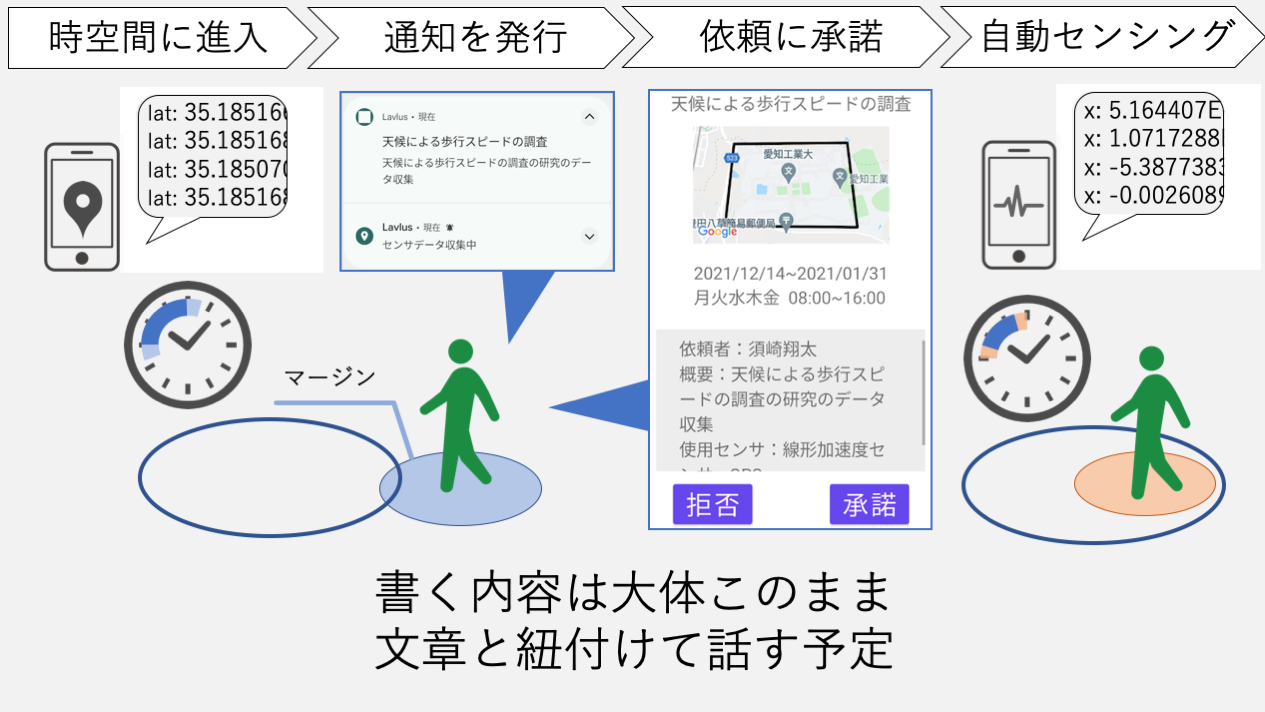
\includegraphics[width=16cm]{img_myApp.png}
    \caption{特定の時空間への進入時に自動センシングするアプリケーションの全体図}
    \label{fig:myApp}
\end{figure}

実装したアプリの全体図を図\ref{fig:myApp}に示す.

\subsection{時空間フェンシングの実装}
\label{myApp_STF}
ジオフェンシングには緯度経度,BLEビーコン,Wi-Fiなどが使われる.
ラヴラスではジオフェンシングを確実に認識する必要がある.
そのため,今回は依頼者と協力者が視覚的に認識しやすい緯度経度を採用した.
% 時空間に進入しているかの判定のため,一定間毎に位置情報を現在時刻を取得する.

ジオフェンスが緯線,経線に並行な線のみでできている長方形の場合,条件分岐を用いてジオフェンシングが可能である.
現在位置の緯度がジオフェンスの最北端よりも低く最南端よりも高い,また経度が指定エリアの最東端よりも低く最西端よりも高い場合,ジオフェンス内にいると判定する.
この条件分岐を用いると,正常にジオフェンシングできるのは緯度経度と平行な辺のみで構成されている矩形のみとなる.
ラヴラスのユースケースとして,特定の施設や建物などを対象とする場合があり,多くの施設や建物は緯度経度に並行ではない.
緯度経度に並行ではない場合,条件分岐では正確なジオフェンシングができない.
例えば,ジオフェンスがひし形の場合を想定する.

\begin{figure}[tbh]
    \centering
    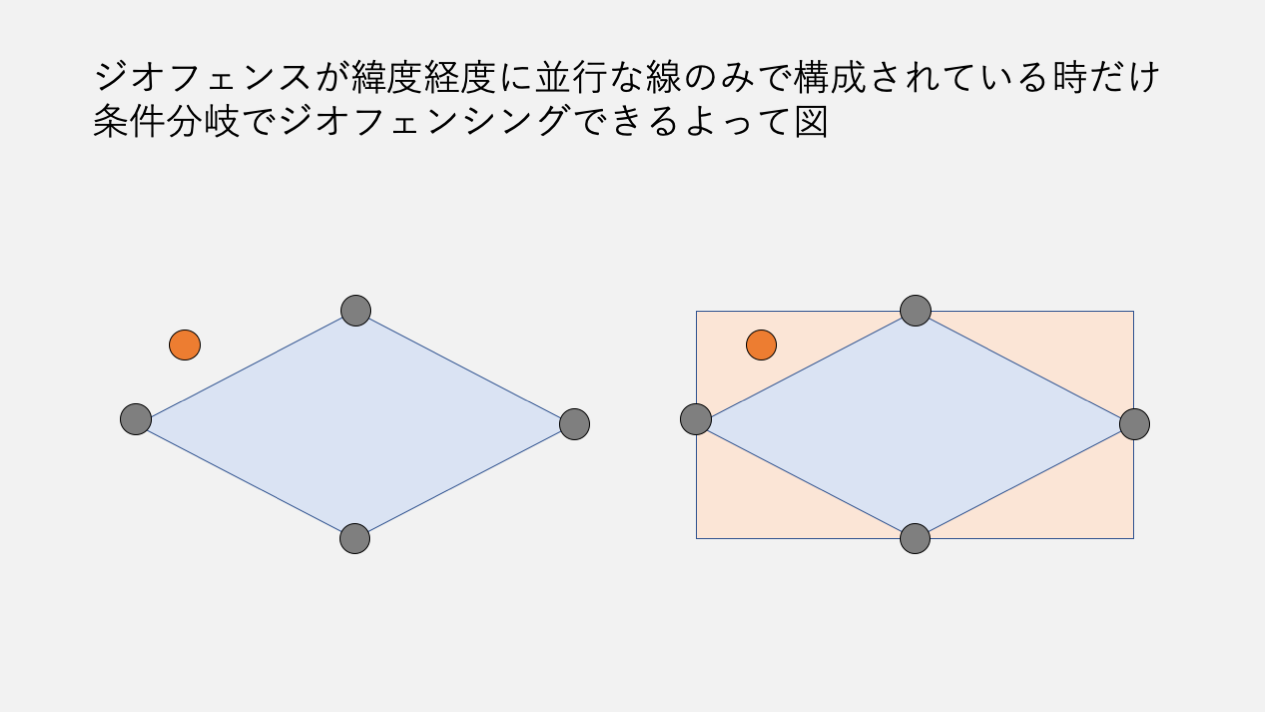
\includegraphics[width=16cm]{img_polygon_1.png}
    \caption{条件分岐を用いたジオフェンシング}
    \label{fig:polygon_1}
\end{figure}

\begin{figure}[tbh]
    \centering
    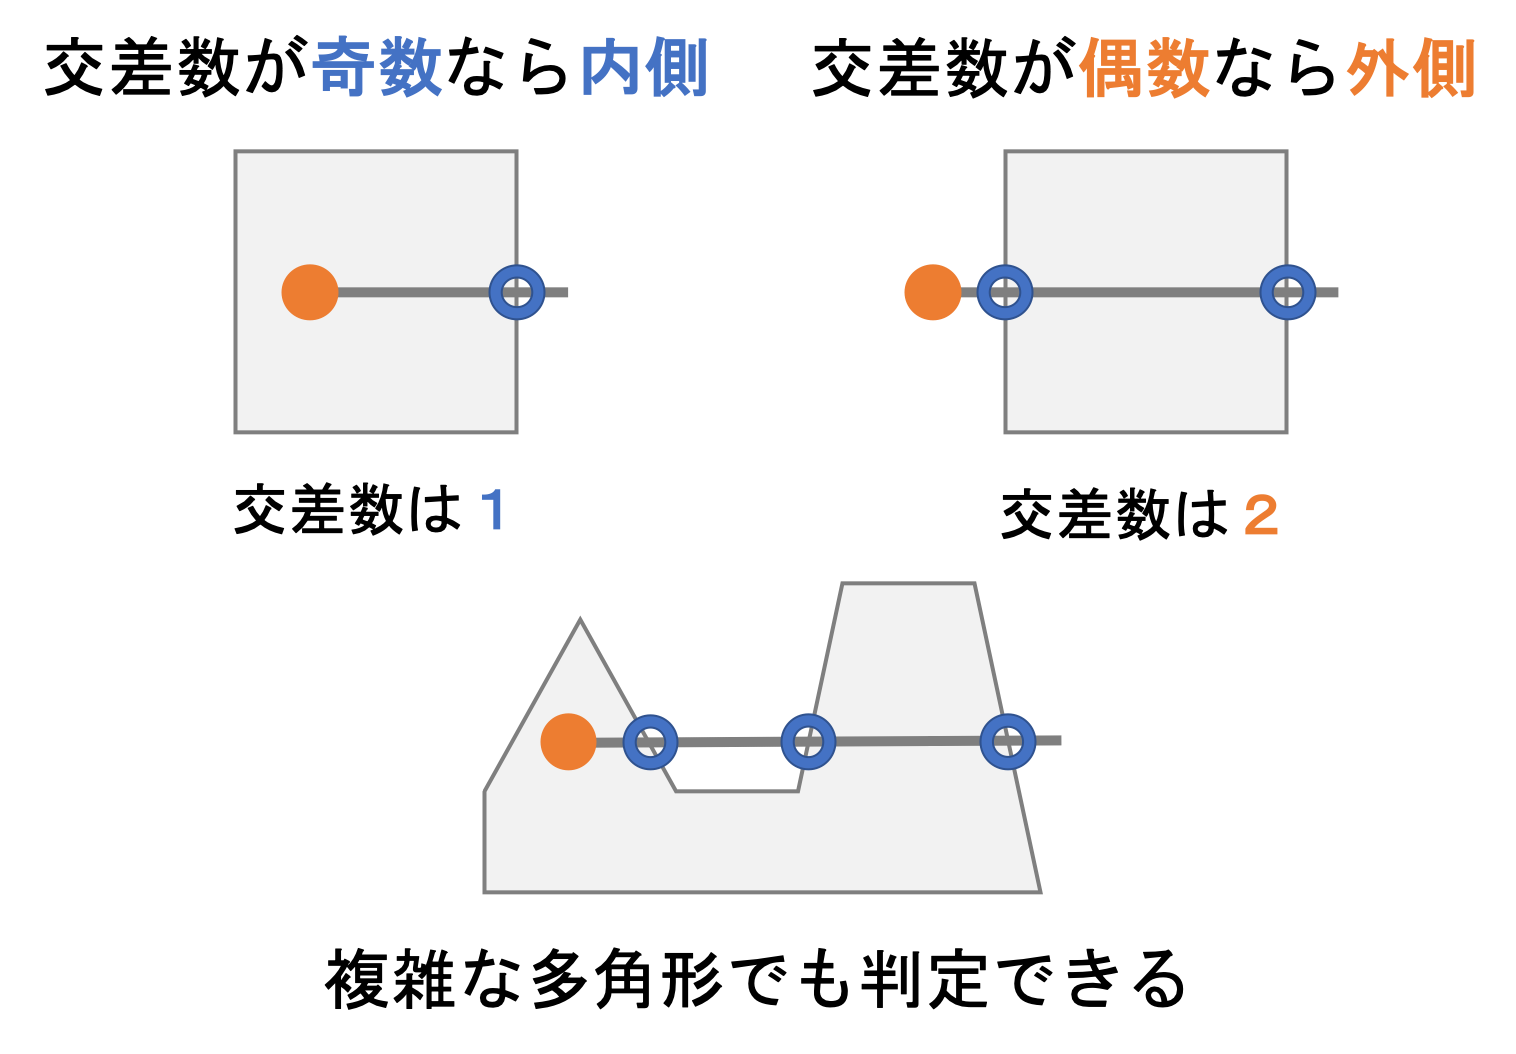
\includegraphics[width=16cm]{img_polygon_2.png}
    \caption{点の内外判定を用いたジオフェンシング}
    \label{fig:polygon_2}
\end{figure}

正常なエリア判定としては,図\ref{fig:polygon_1}左の通り現在地(赤丸)にいた場合はエリア内に進入していないため,通知は送られないはずである.
しかし,条件分岐を用いたエリア判定の場合は,ひし形の外側にひし形の頂点を辺の中心とした矩形の判定エリアが形成されるため,図\ref{fig:polygon_1}右のように現在地がエリア内にいると判定され,誤って通知が送られてしまう.
このように,条件分岐を用いると自ずとジオフェンスが矩形になってしまう.

ジオフェンスが複雑な矩形な場合に対応するためにポリゴンの内外判定アルゴリズム\cite{naigai}を使用する.
点の多角形に対する内外判定を図\ref{fig:polygon_2}に示す.
点の内外判定とは,まず点(青丸)から多角形に対して線を引く.
この時引く線は直線であれば,どの方向に引いても良い.
その線と多角形との交点(赤丸)の数が奇数個であれば多角形よりも内側にいる,偶数個であれば多角形よりも外側にいると判定できる.
この場合,丁度線と多角形の辺が重なったり,線と多角形の頂点と重なると,誤った判定を行ってしまう.
しかし,緯度経度は小数点以下が7桁もあり,位置情報は変化し続けるため,丁度重なる場合は今回考えないものとしている.
依頼者が図\ref{fig:polygon_2}のようにどれだけ複雑な多角形のエリアを設定しても,内部か否かは判定可能である.
今回は実装は行っていないが円のようなエリアでも判定は可能である.
また,今回はGPSのみを用いたエリア判定のため,平面的なエリア判定しか行えない.
1階や2階などの立体的なエリア判定は今後の課題とする.

確実に時空間に進入した場合のみセンシングする,時空間に進入する可能性が高い協力者にセンシング依頼通知を発行するなど,様々なシチュエーションに対応するため,時空間の拡大と縮小が可能なマージンを実装した.

\begin{figure}[tbh]
    \centering
    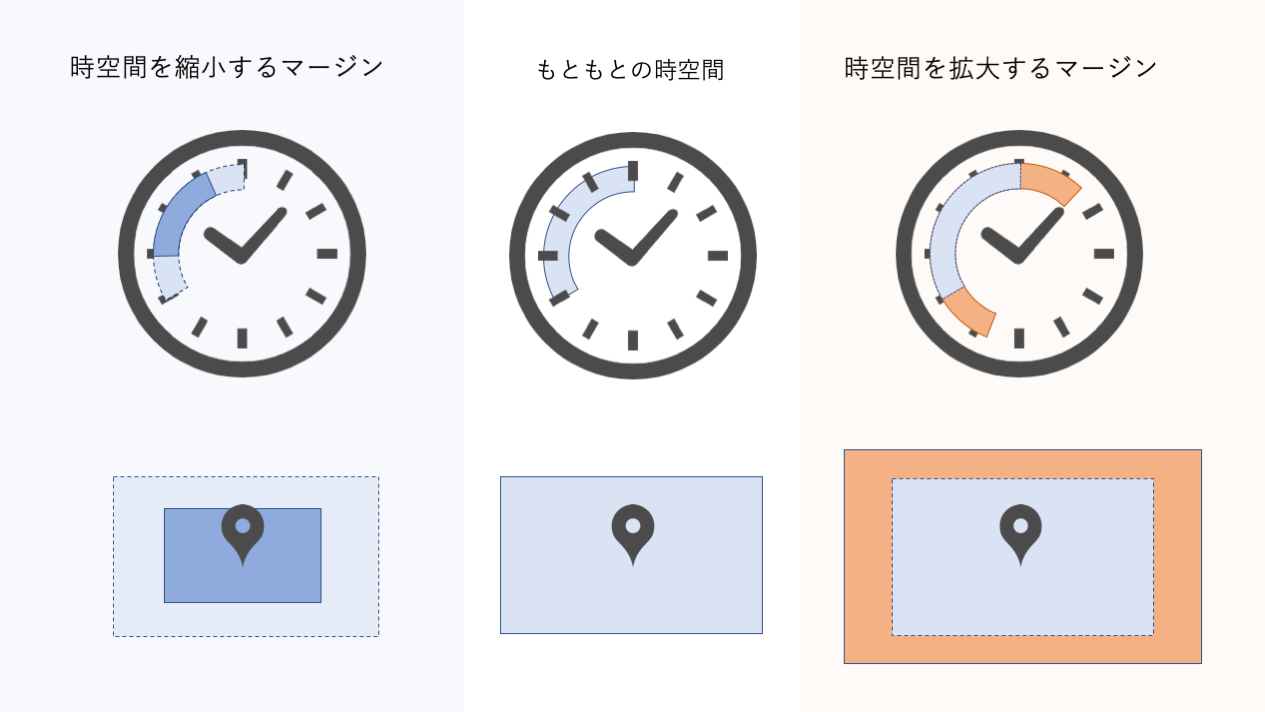
\includegraphics[width=16cm]{img_margin_1.png}
    \caption{時空間を拡大縮小するマージンの例}
    \label{fig:margin_1}
\end{figure}

時空間を拡大縮小するマージンの例を図\ref{fig:margin_1}に示す.
ジオフェンスが緯線,経線に並行な線のみでできている長方形の場合,加算と減算を用いてマージンの実装が可能である.
ジオフェンスを拡大する場合は,最北端の緯度と最東端の経度に加算し最南端の緯度と最西端の経度に減算する.
ジオフェンスを縮小する場合は,最北端の緯度と最東端の経度に減算し最南端の緯度と最西端の経度に加算する.
しかし,本アプリはジオフェンスが複雑な矩形に対応する必要がある.
ジオフェンスが複雑な矩形の場合に対応するため,ジオフェンスではなく協力者にマージンを持たせた.

\begin{figure}[tbh]
    \centering
    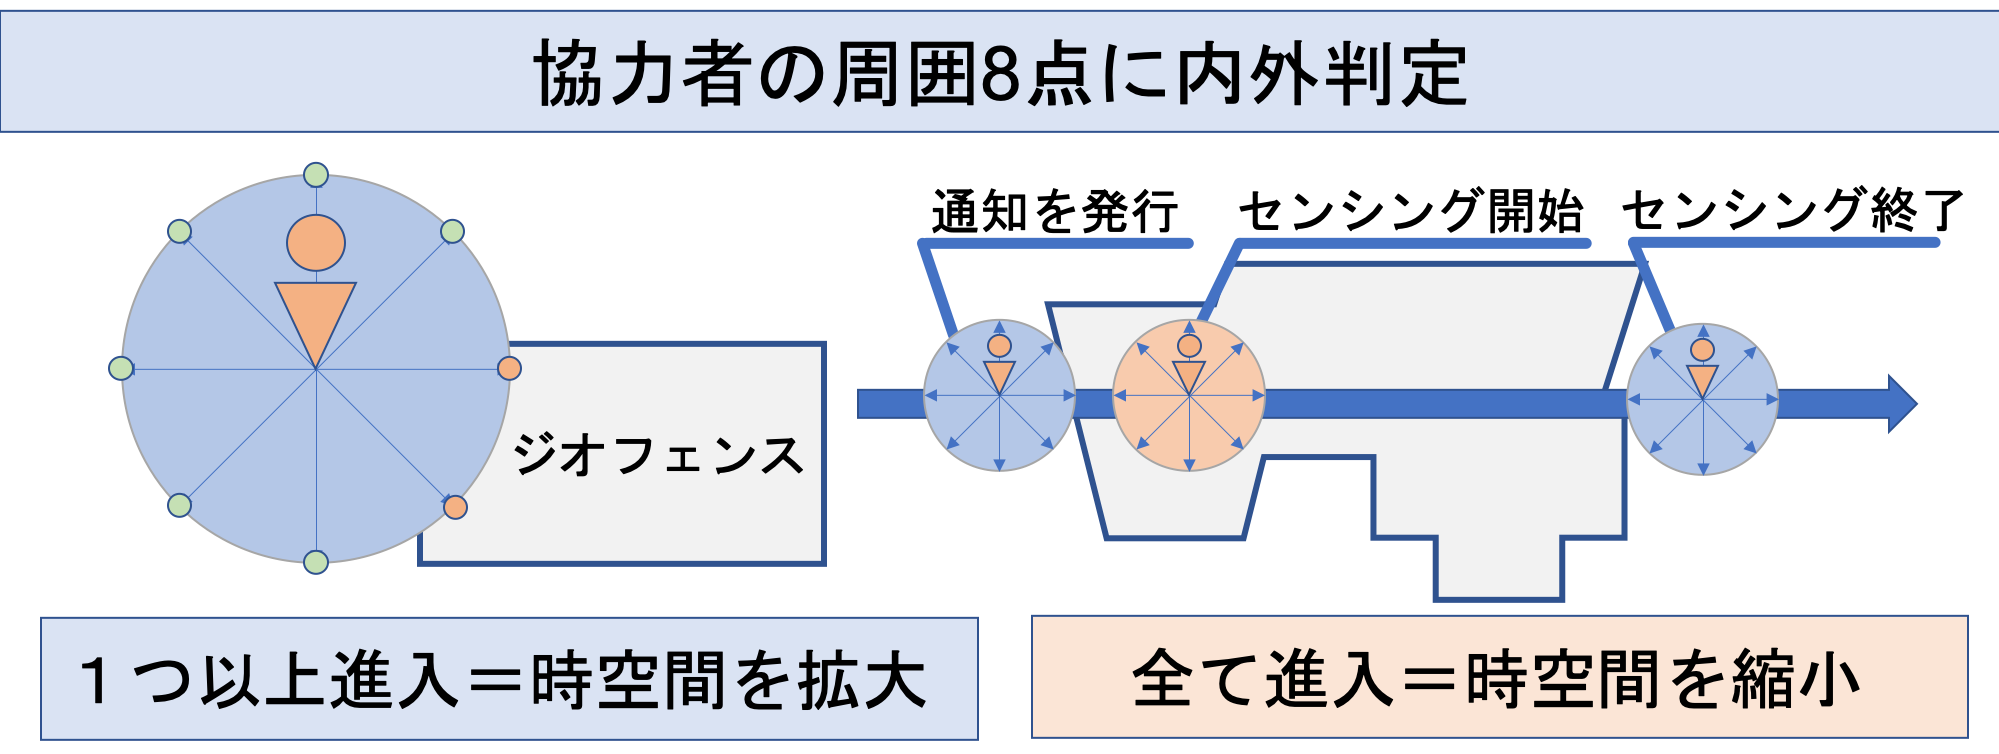
\includegraphics[width=16cm]{img_margin_2.png}
    \caption{時空間を拡大縮小するマージン}
    \label{fig:margin_2}
\end{figure}

協力者に対するマージンを図\ref{fig:margin_2}に示す.
協力者の現在位置から上下左右斜めに8つの点を作る.
ジオフェンスを拡大する場合は,8つの点のうち1つでもジオフェンシングに進入している時に進入していると判定する.
ジオフェンスを縮小する場合は,8つの点が全てジオフェンシングに進入している時に進入していると判定する.
これにより,どれだけ複雑な矩形でもマージンを持たせられる.

% ジオフェンスに緯度経度を使用しているため,ジオフェンスのマージンの距離を緯度経度に変換する必要がある.


% 緯度経度の距離の話,複雑な矩形の話,


% 複雑な矩形のマージンに対応できるように端末にマージンを設けた.

\subsection{センシング依頼通知の実装}
\label{myApp_notify}
協力者へのセンシング依頼通知を減らすために,センシング依頼通知はクラウドセンシングに参加する可能性が高い協力者に発行する.
センシングプロジェクトに設定された時空間に近い協力者を,そのクラウドセンシングに参加する可能性が高いとする.
例えば,すでに始まっているクラウドセンシングの付近にいる協力者や,もうすぐ自分がいる場所でクラウドセンシングが始まる協力者である.
なので,時空間を広げるようにマージンを取り,その時空間へ進入した場合,通知を発行する.
センシングプロジェクトに設定された空間から離れた場所にいる協力者はそのクラウドセンシングに参加する可能性が低いとする.
例えば,すでに始まっているクラウドセンシングから離れた場所にいる協力者である.
クラウドセンシングに参加する可能性が低い協力者に通知を発行しても,クラウドセンシングに参加する可能性が低く,たとえセンシング依頼に承諾しても,センサデータがもらえる可能性が低い.
また,協力者は参加しないクラウドセンシングの通知が何度も発行されると不快に感じる可能性がある.
すでにジオフェンスに進入していても,数日後や数ヶ月後など大きく時間が離れている場合も通知を発行しない.
旅行や出張などで遠出している協力者が旅行先で,数ヶ月後に行われるクラウドセンシングの通知を受け取っても参加する可能性が低い.
自宅や職場の付近で,数ヶ月後に行われるクラウドセンシングは,協力者が参加する可能性が低くない.
しかし,普段から設定されたジオフェンスに近づく場合,そもそもクラウドセンシングに参加する可能性が高いため,数日前,数ヶ月前に通知を発行する必要はない.
また,センシング依頼に承諾してから数日すると,協力者は承諾したクラウドセンシングについて忘れる可能性がある.

\begin{figure}[tbh]
    \centering
    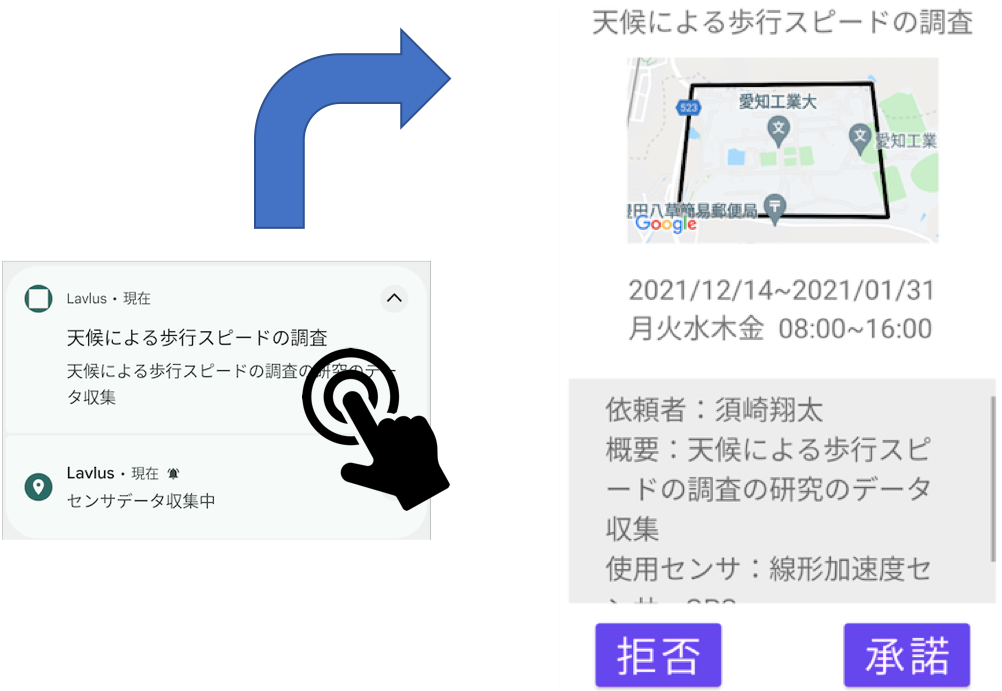
\includegraphics[width=16cm]{img_notify.png}
    \caption{発行される通知とセンシング依頼画面の例}
    \label{fig:notify}
\end{figure}


協力者がセンシング依頼通知をタップすると,センシング依頼画面が立ち上がり,依頼者の名前や使用するセンサ,時空間が提示される(図\ref{fig:notify}).
協力者に対するジオフェンスの提示はAndroidアプリと親和性の高いGoogleMapを使用している.
協力者がセンシング依頼通知を開いた時,ジオフェンスを瞬時に認識するために,GoogleMapにジオフェンスの境界線を引き,GoogleMapのズームレベルを調整している.
GoogleMapはジオフェンスの中央を中心に表示されている.
ジオフェンスの中央の緯度は最北端と最南端,経度は最東端と最西端の平均から求めている.
GoogleMapはジオフェンスを全て表示するズームレベルに設定される.
最北端と最南端から縦の長さ,最東端と最西端から横の長さを計算し,ズームレベル毎のピクセルと距離の関係\cite{GoogleMap}を参考に適切なズームレベルを算出する.

協力者が提示された情報に納得し協力すると判断した場合,協力者はセンシング承諾ボタンを押してクラウドセンシングに協力する.
協力者はセンシング依頼画面に提示される情報を確認する.
この時,協力者は提示された情報に少しでも不信感を覚えたり,納得できない場合はセンシング拒否ボタンを押してクラウドセンシングに協力しない.



\subsection{自動センシングの実装}
\label{myApp_sensing}
% 入った時と出た時でマージンが違う.
% どう言った時でセンシングが始まるべきか,おわるべきか.
協力者の操作を低減させる為,協力者が時空間に進入し,センシング依頼に承諾している場合,バックグラウンドで自動にセンシングされる.
そのため,協力者はスマホアプリを意識して開く必要はなく,アプリケーション自体を終了させなければ,途中でセンシングは終了しない.
バックグラウンドにより,協力者の操作などの負担の軽減に加え,センシングをしているという感覚を意識させないため,より普段の振る舞いをセンシングできる.

確実に協力者の時空間への進入,退出を判定するため,進入時は時空間を狭くするマージン,退出時は時空間を広くするマージンを取る.
ジオフェンシングの境界付近かつ,位置情報が不安定になると進入,退出の判定を繰り返してしまう.
これを防ぐためにマージンを取る.
しかし,時空間が小さい場合,狭くするマージンを取りすぎると時空間に進入しづらく,または進入できなくなってしまう.
例えば縦横どちらかが10m以下のジオフェンスに対して狭くするマージンを5m以上取ると進入できなくなる.
同様に時間を狭くするマージンを設定された時間より多くとってしまうと進入できなくなる.
そのため時空間を狭くするときのマージンは時空間の大きさを考慮する必要がある.
現時点でマージンはセンシングプロジェクト毎に設定している.

クラウドセンシングプラットフォームとして多くのセンサと自由な周波数に対応し,プライバシを侵害するセンサデータは抽象化した.
さまざまなクラウドセンシングに対応するために多くのセンサと周波数に対応する必要がある.
例えば,歩行推定では加速度センサ,気圧センサ,角速度センサ,位置情報などが必要になる可能性がある.
騒音計測では音センサ,環境測定では温度や湿度が必要になる可能性がある.
センサの種類だけではなく,自由に設定できる周波数も必要である.
同じセンサでも,用途によって周波数はさまざまである.
例えば,気圧センサを歩行推定に使う場合,高い周波数でセンシングする.
一方,天候推定では高い周波数でセンシングする必要がないため,低い周波数でセンシングする.
依頼者が作成するセンシングプロジェクトにはセンサの種類とセンサ毎の周波数が設定されている.
本アプリではセンシングプロジェクトに沿って,複数のセンサとセンサ周波数に対応したセンシングができる.
例えば,加速度を50Hz,気圧を10Hzでセンシングなど,周波数をセンサ単位で設定できる.
また,同時に複数の時空間に進入して,複数のクラウドセンシングに参加する場合がある.
本アプリはセンシングプロジェクト毎にセンサの種類とその周波数を管理しているため,同時に複数のセンシングが可能である.
例えば,加速度を50Hzで取るクラウドセンシグと20Hzでとるクラウドセンシングに協力した場合でも適当にセンシングできる.


% その為,プライバシを侵害する可能性が高いセンサデータは抽象化されている.
% ジオフェンシングの境界付近かつ,位置情報が不安定になると進入,退出の判定を繰り返してしまう.


% Local Variables: 
% mode: japanese-LaTeX
% TeX-master: "root"
% End: 


\chapter{動作検証}
\thispagestyle{myheadings}
本研究の動作検証は特定の時空間に進入時のみセンシングできているか,プラットフォームとして複数のユースケースを想定して適切にセンシングできているかの2つを行う.

\section{時空間フェンシングの動作検証}
% 目的,環境,結果,考察
ジオフェンスが複雑な矩形の時,マージンを含め適切に動作しているか検証した.
拡大したジオフェンスに進入した時に通知を発行し,縮小したジオフェンスに進入した時にセンシングが始まり,拡大したジオフェンスから退出した時にセンシングが終了していれば適切に動作しているとする.
動作検証の設定は図\ref{fig:ex_margin_1}に示す.

\begin{figure}[tbh]
    \centering
    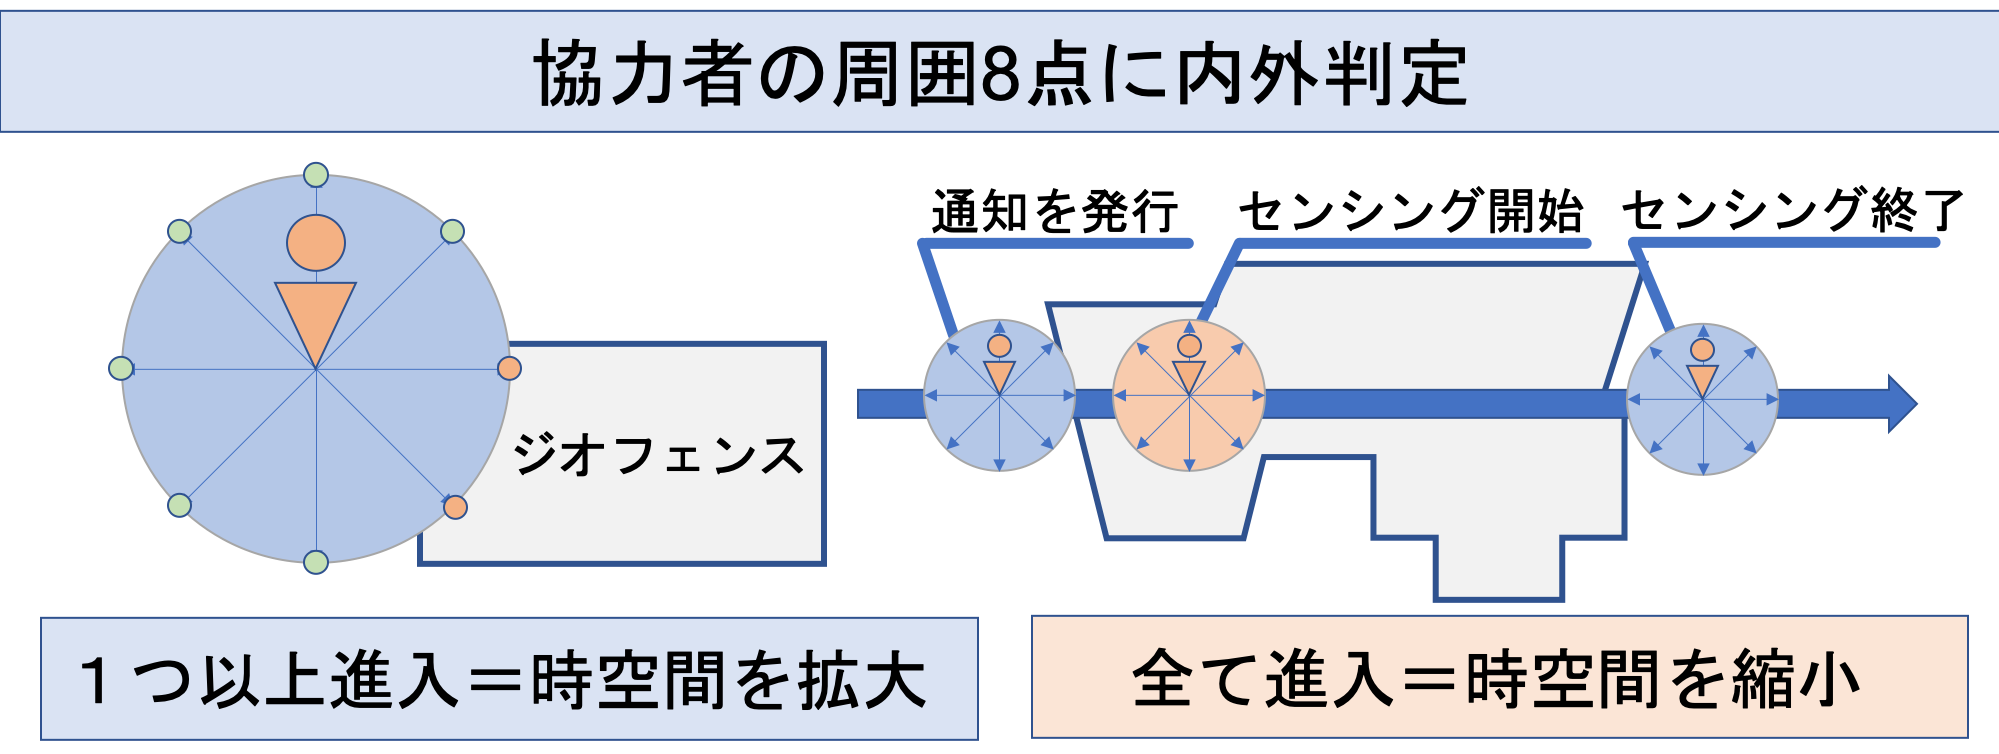
\includegraphics[width=16cm]{img_margin_2.png}
    \caption{時空間を拡大縮小するマージン}
    \label{fig:ex_margin_1}
\end{figure}

結果適切な動作が確認できた.
% (屋内でもやる)

\section{ユースケースを想定した動作検証}
まず,天候によって所要時間が変化する地図アプリを作成したい人がいたと仮定する.
時空間を歩行者の多い8時30分から16時50分の愛知工業大学と設定し,使用するセンサを線形加速度とGPSとした(図\ref{fig:ex_case_1}).

\begin{figure}[tbh]
    \centering
    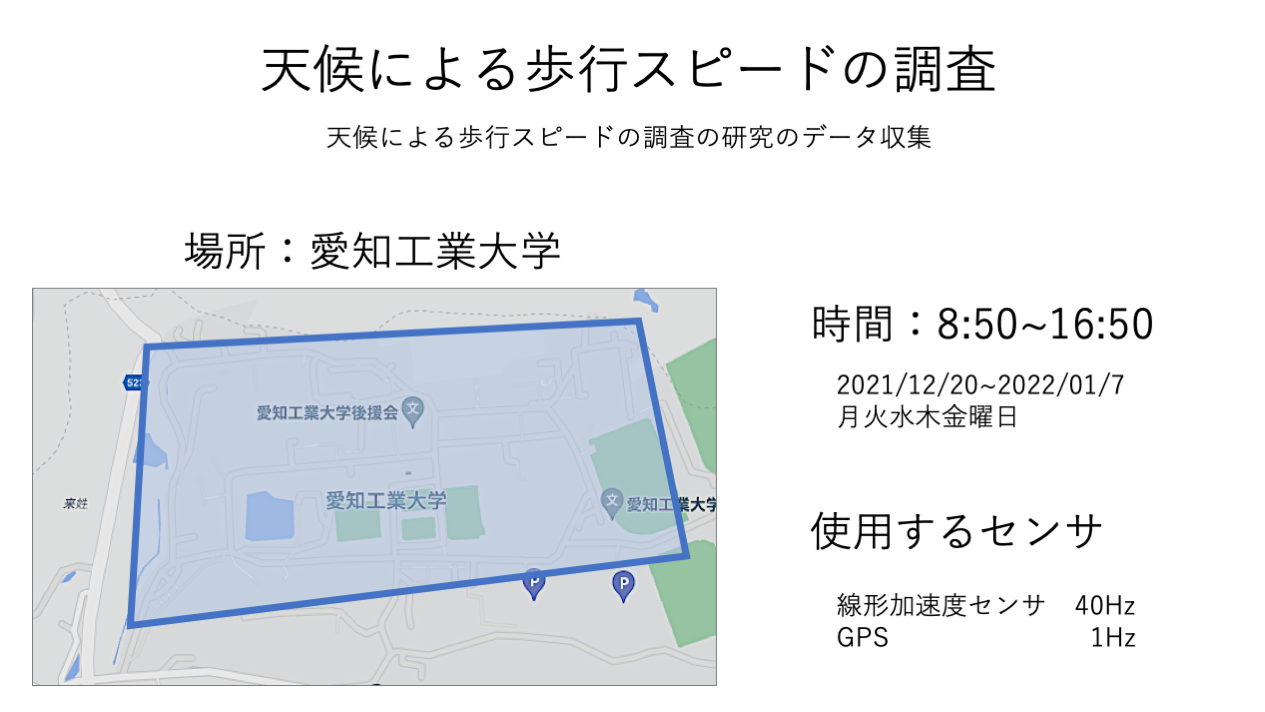
\includegraphics[width=16cm]{img_ex_case_1.png}
    \caption{天候によって所要時間が変化する地図アプリのためのクラウドセンシング}
    \label{fig:ex_case_1}
\end{figure}

結果,集めたセンサデータから移動速度と歩幅推定などができた.

次に,研究室の管理者が,研究室内でどれだけコミュニケーションが取られているか測定しようとしたと仮定する.
時空間を滞在者の多い8時30分から16時50分の研究室と設定し,使用するセンサを音センサとした.

\begin{figure}[tbh]
    \centering
    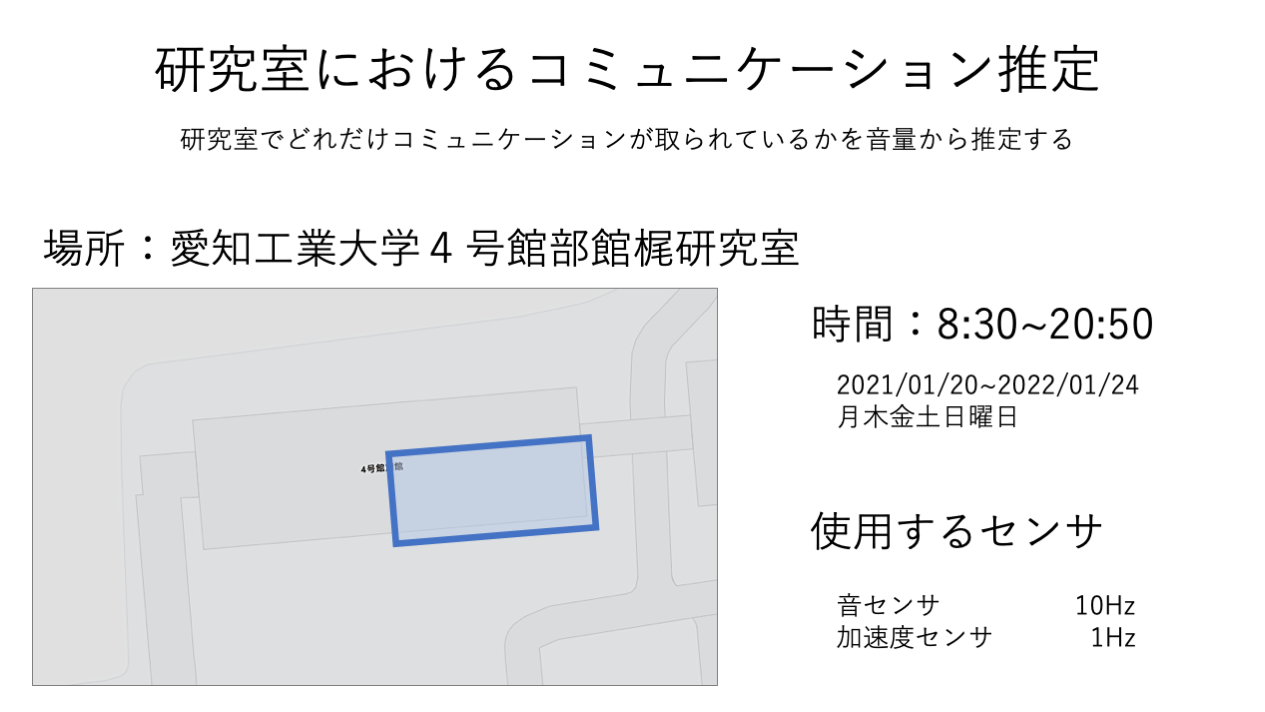
\includegraphics[width=16cm]{img_ex_case_2.png}
    \caption{天候によって所要時間が変化する地図アプリのためのクラウドセンシング}
    \label{fig:ex_case_2}
\end{figure}

結果,集めたセンサデータから時間帯ごとの賑やかさが推定できた.

% Local Variables: 
% mode: japanese-LaTeX
% TeX-master: "root"
% End: 


\chapter{おわりに}
\thispagestyle{myheadings}

\section{まとめ}
本研究では協力者のディスインセンティブ要素を軽減し,ユーザのセンシングの協力かつ継続を促した.
動作検証では時空間フェンシングが適切に行えているか確認した.その結果時空間フェンシングが適切に行えた.
実際のユースケースを想定して適切にセンシングできているか検証した.その結果さまざまなセンサデータを集められた.

\section{今後の課題}
今後の課題として,今回実装に至らなかった時空間フェンシングに基づくクラウドセンシングプラットフォームにおけるモバイルアプリケーションに必要な機能の実装が挙げられる.
時空間フェンシングにGPSを使用しているのでGPSの精度が落ちる屋内で動作が不安定になる点.


% Local Variables: 
% mode: japanese-LaTeX
% TeX-master: "root"
% End: 


\chapter*{謝辞}
\addcontentsline{toc}{chapter}{\protect\numberline {} 謝辞}

本研究を進めるにあたり,多くの御指導,御鞭撻を賜わりました
梶克彦准教授に深く感謝致します.

梶研究室に所属された当初,私には髪がありませんでした.
1つ上の先輩達から怖がられたりしましたが,サマーワークショップでは新規性とは,デザインとは,スケジューリングなど御教授賜りました.
サマーワークショップ後は本研究とは別に,React.jsを使ってWebアプリ作成を教えてもらいました.
この時コールバックやデザイン,APIの知識を教えてもらい,今でも教えてもらってよかったと思っております.

あの頃と比べて髪もだいぶ長くなりました.
わざわざ有給と取り1ヶ月に一度研究室を訪れてくださる,言わば妖精とも言える先輩を中心にOBの先輩達からとてもお世話になりました.
彼を中心に作られたSlackチャンネルで今でも繋がっております.
アプリ開発中どうしても理解できなかった部分に関して,OBの先輩に質問した時とても詳細で的確な回答とアドバイスをもらいました.
また,本論の図や文章に対しても多くのコメントを送っていただきました.
先輩達がいなかったら,今の私はいなかったと思います.
卒業した後でも面倒を見てくれる先輩達に深く感謝いたします.

私の行動範囲を広げ,移動時間を大幅に短縮してくれた老人マーク,身体障害者マークのついた赤いプリウスに感謝します.

卒論執筆中私の精神安定剤になってくれた,インスタントコーヒーのブレンディと1年以上消費期限の切れたネスカフェゴールドに感謝します.

最後に,日頃から熱心に討論,助言してくださいました
梶研究室のみなさんに深く感謝致します.


% Local Variables: 
% mode: latex
% TeX-master: "root"
% End: 


\thispagestyle{myheadings}
\addcontentsline{toc}{chapter}{\protect\numberline {} 参考文献}

\bibliography{reference}
\bibliographystyle{junsrt}
% Local Variables: 
% mode: japanese-LaTeX
% TeX-master: "root"
% End: 


% これ以降,付録となる
\appendix

\end{document}
